\documentclass[letterpaper, 12pt]{article}
% \usepackage[showframe, margin=1in, top=0.25in, bottom=0.25in, includeheadfoot, headheight=0.5in]{geometry}
\usepackage[margin=1in, top=0.25in, bottom=0.25in, includeheadfoot, headheight=0.5in]{geometry}

\AddToHook{cmd/section/before}{\clearpage}

\usepackage[table]{xcolor}
\colorlet{listingback}{gray!20}
\definecolor{headingcolor}{RGB}{110,34,54}

\usepackage{fancyhdr}
\renewcommand{\sectionmark}[1]{\markboth{#1}{#1}}

% Used to detect whether a section is an appendix to print the right thing in the footer
\usepackage{etoolbox}
\newtoggle{inappendix}
\pretocmd{\appendix}{\clearpage\toggletrue{inappendix}}{}{}

% Save standard definitions for head and foot rules (lines separating header and footer from text)
\let\HeadRule\headrule
\let\FootRule\footrule
% Add color to the standard definitions
\renewcommand{\headrule}{\color{headingcolor}\HeadRule}
\renewcommand{\footrule}{\textcolor{headingcolor}{\FootRule}}

% IMPORTANT: This command should not be called directly. Use \preamble.
% Macro to insert the title page for each lab.
% The argument is the title of the lab.
\newcommand{\inserttitlepage}[1]
{
    \begin{titlepage}
    \centering
    
\includegraphics[scale=0.5]{images/nexus_lab_logo.png}

    \vspace*{\baselineskip}

    \textbf{\Large OpenStack Labs}

    \vspace*{\baselineskip}

    \textbf{\Large #1}
    \vspace*{\fill}
\end{titlepage}
}

% IMPORTANT: This command should not be called directly. Use \preamble.
% Macro to define header and footer for each lab.
% The argument is the title of the lab.
\newcommand{\headfoot}[1]
{
    \fancypagestyle{fancy}
    {
        \fancyhf{}
        \fancyhead[L]{\footnotesize #1}
        \fancyhead[R]{
\includegraphics[height=0.85\headheight]{images/nexus_lab_logo.png}}
        \fancyfoot[L]{%
            \footnotesize%
            \ifnum\value{section}>0%
            \iftoggle{inappendix}{Appendix \thesection: \rightmark}{Section \thesection: \rightmark}%
            \fi}
        \fancyfoot[R]{\footnotesize\thepage}
        \renewcommand{\headrulewidth}{1.5pt}
        \renewcommand{\footrulewidth}{1.5pt}
    }
}

% Macro to insert title page, define header and footer, and insert table of contents and about section for each lab.
% The argument is the title of the lab.
\newcommand{\preamble}[1]
{
    \pagenumbering{roman}
    \inserttitlepage{#1}
    \headfoot{#1}

    % Insert table of contents
    \pagestyle{fancy}
    \tableofcontents
    \clearpage

    \section*{About This Document}
    \label{sec:about_this_document}
    \begin{itemize}
        \item This document was developed by a team at the University of Tennessee at Chattanooga led by Dr. Mengjun Xie
        (\href{mailto:mengjun-xie@utc.edu}{\textbf{mengjun-xie@utc.edu}}).
        \item The development of this document was supported by a National Centers of Academic Excellence in Cybersecurity Grant (\#H98230-20-1-0351), housed at the National Security Agency.
        \item This document is licensed with a Creative Commons Attribution 4.0 International License.
    \end{itemize}
    \clearpage
}

% Macro to insert the Lab Settings page for each lab. Call after the Introduction and Objectives sections.
\newcommand{\labsettings}
{
    \section*{Lab Settings}
    \label{sec:lab_settings}
    \addcontentsline{toc}{section}{\nameref{sec:lab_settings}}
    The information in the table below will be needed in order to complete the lab.
    The task sections below provide details on the use of this information.
    \begin{table*}[htbp]
        \centering
        \begin{tabular}{|c|c|c|c|}
            \hline
            \rowcolor{gray!20} \textbf{Virtual Machine} & \textbf{IP Address} & \textbf{Account} & \textbf{Password} \\
            \hline
            \multirow{2}{*}{\texttt{workstation}} & \multirow[t]{2}{*}{\texttt{ens3: 192.168.1.21}}  & \multirow{2}{*}{\texttt{ubuntu}} & \multirow{2}{*}{\texttt{ubuntu}} \\
                                                  & \multirow[t]{2}{*}{\texttt{ens4: 172.25.250.21}} &                                  &                                  \\
            \hline
            \multirow{2}{*}{\texttt{devstack}}    & \multirow[t]{2}{*}{\texttt{ens3: 192.168.20}}    & \multirow{2}{*}{\texttt{ubuntu}} & \multirow{2}{*}{\texttt{ubuntu}} \\
                                                  & \multirow[t]{2}{*}{\texttt{ens4: 172.25.250.20}} &                                  &                                  \\
            \hline
        \end{tabular}
    \end{table*}
    \clearpage

    % IMPORTANT(lucas): If another frontmatter section ever gets placed after this, this command needs to be moved
    % to the end of that section.
    % I have placed this here and not in each lab purely for convenience and to ensure I don't forget any.
    \pagenumbering{arabic}
}

% Sans-serif font
\renewcommand{\familydefault}{\sfdefault}
\newcommand{\texttildemid}{{\raisebox{0.5ex}{\texttildelow}}}

\usepackage{enumitem}
\renewcommand{\labelenumi}{\textbf{\thesection.\arabic{enumi}.}}

% Try to forbid widows and orphans
\widowpenalty10000
\clubpenalty10000

\usepackage{graphicx}
\usepackage{hyperref}
\hypersetup{colorlinks=true,linkcolor=black,urlcolor={[named] headingcolor}}

\usepackage{sectsty}
\sectionfont{\color{headingcolor}}

% Table of Contents
\usepackage{bookmark}
\usepackage[titles]{tocloft}
\usepackage[title]{appendix}
\renewcommand{\cfttoctitlefont}{\Large\bfseries\color{headingcolor}}
\renewcommand{\cftsecfont}{\normalfont\normalsize}
\renewcommand{\cftsecpagefont}{\normalfont\normalsize}
\renewcommand{\cftdotsep}{0} % Make dots small and close together
\renewcommand{\cftsecleader}{\cftdotfill{\cftdotsep}} % Add dots after section titles
% Make dots go all the way to the page number
\renewcommand{\cftsecfillnum}[1]{{\cftsecleader}\nobreak{\cftsecpagefont #1}\cftsecafterpnum\par}

\usepackage{multirow}
\setlength{\tabcolsep}{16pt}
\renewcommand{\arraystretch}{1.1}

% For nice-looking boxes
\usepackage[most]{tcolorbox}
\usepackage{listings}
\usepackage{lstautogobble}
\lstset{
  frame=none,
  language=Bash,
  showstringspaces=false,
  basicstyle={\linespread{1.1}\footnotesize\ttfamily\selectfont},
  numbers=none,
  breaklines=true,
  breakatwhitespace=true,
  tabsize=3,
  columns=fullflexible,
  keepspaces=true,
  escapeinside={(*@}{@*)},
  literate={~}{{\texttildemid}}{1}
           {\#}{\#}{1},
  autogobble=true
}

\tcolorboxenvironment{lstlisting}
{
    spartan,
    colframe=gray!50,
    boxsep=0mm,
    left=1mm,
    right=1mm,
    top=-1mm,
    bottom=-1mm,
    colback=gray!20
}

% Hacky solution for now, would like to have just one environment and make several tcolorboxes by passing different
% colors as parameters, but that is giving errors
\makeatletter
\tcbset{
  note/.style={%
        enhanced,
        breakable,
        colback=blue!10!white,
        colframe=blue!80!white,
        attach boxed title to top left={yshift*=-\tcboxedtitleheight},
        title={#1},
        boxed title size=title,
        boxed title style={%
            sharp corners,
            rounded corners=northwest,
            colback=tcbcolframe,
            boxrule=0pt,
        },
        underlay boxed title={%
            \path[fill=tcbcolframe] (title.south west)--(title.south east)
                to[out=0, in=180] ([xshift=5mm]title.east)--
                (title.center-|frame.east)
                [rounded corners=\kvtcb@arc] |-
                (frame.north) -| cycle;
        },
    }
}
\makeatother

\makeatletter
\tcbset{
    stop/.style={%
        enhanced,
        breakable,
        colback=white,
        colback=red!10!white,
        colframe=red!80!white,
        attach boxed title to top left={yshift*=-\tcboxedtitleheight},
        title={#1},
        boxed title size=title,
        boxed title style={%
            sharp corners,
            rounded corners=northwest,
            colback=tcbcolframe,
            boxrule=0pt,
        },
        underlay boxed title={%
            \path[fill=tcbcolframe] (title.south west)--(title.south east)
                to[out=0, in=180] ([xshift=5mm]title.east)--
                (title.center-|frame.east)
                [rounded corners=\kvtcb@arc] |-
                (frame.north) -| cycle;
        },
    }
}
\makeatother

\makeatletter
\tcbset{
    tip/.style={%
        enhanced,
        breakable,
        colback=white,
        colback=green!10,
        colframe=green!70!black,
        attach boxed title to top left={yshift*=-\tcboxedtitleheight},
        fonttitle=\bfseries,
        title={#1},
        boxed title size=title,
        boxed title style={%
            sharp corners,
            rounded corners=northwest,
            colback=tcbcolframe,
            boxrule=0pt,
        },
        underlay boxed title={%
            \path[fill=tcbcolframe] (title.south west)--(title.south east)
                to[out=0, in=180] ([xshift=5mm]title.east)--
                (title.center-|frame.east)
                [rounded corners=\kvtcb@arc] |-
                (frame.north) -| cycle;
        },
    }
}
\makeatother

% The commands below define environments for colored boxes. They are used like
% \begin{notebox}
% ...
% \end{notebox}
\newtcolorbox{notebox}{note={Note}}
\newtcolorbox{stopbox}{stop={Stop}}
\newtcolorbox{tipbox}{tip={Tip}}

\begin{document}
\preamble{Lab 04: Deploying an External Instance}

\section*{Introduction}
\label{sec:introduction}
\addcontentsline{toc}{section}{\nameref{sec:introduction}}
Up to this point, everything you have worked on has been local to the OpenStack environment. In this lab, you will learn
the various concepts necessary to give OpenStack instances and networks external connectivity. You will manage external
networks, routers, and floating IP addresses to give OpenStack instances and networks external connectivity; SSH key
pairs to allow you to connect to an OpenStack instance from outside the OpenStack environment; and security groups to
prevent unwanted traffic in the network. These resources will come together to allow OpenStack instances to provide
services outside of the OpenStack cloud and allow you to manage instances from outside the cloud.

\section*{Objectives}
\label{sec:objectives}
\addcontentsline{toc}{section}{\nameref{sec:objectives}}
\begin{itemize}[itemsep=0pt]
    \item Manage external networks.
    \item Manage OpenStack routers.
    \item Manage floating IP addresses.
    \item Manage SSH key pairs.
    \item Manage security groups.
    \item Launch and verify an external instance.
\end{itemize}
\clearpage

\labsettings

%%%%%%%%%%%
% Section 1
%%%%%%%%%%%
\section{Managing External Networks}
\label{sec:managing_external_networks}
In this task, you will use the \textit{Horizon Dashboard} and the \textbf{OpenStack Unified CLI} to create and configure
an external network.

\begin{enumerate}
    \item Log into the \textbf{workstation} machine as the \textbf{ubuntu} user with password \textbf{ubuntu}.

    \begin{center}
        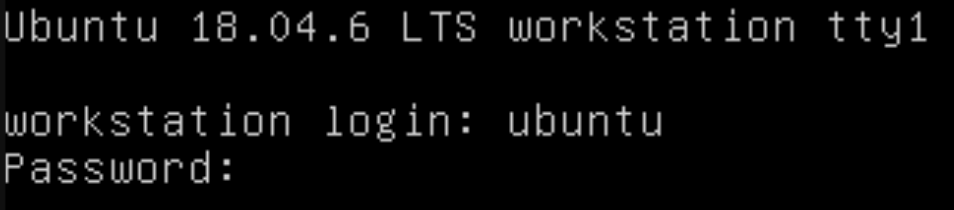
\includegraphics[width=\linewidth]{images/part1/step1.png}
    \end{center}

    \item Launch the graphical user interface.
    \begin{lstlisting}
        ubuntu@workstation:~$ startx
    \end{lstlisting}

    \begin{center}
        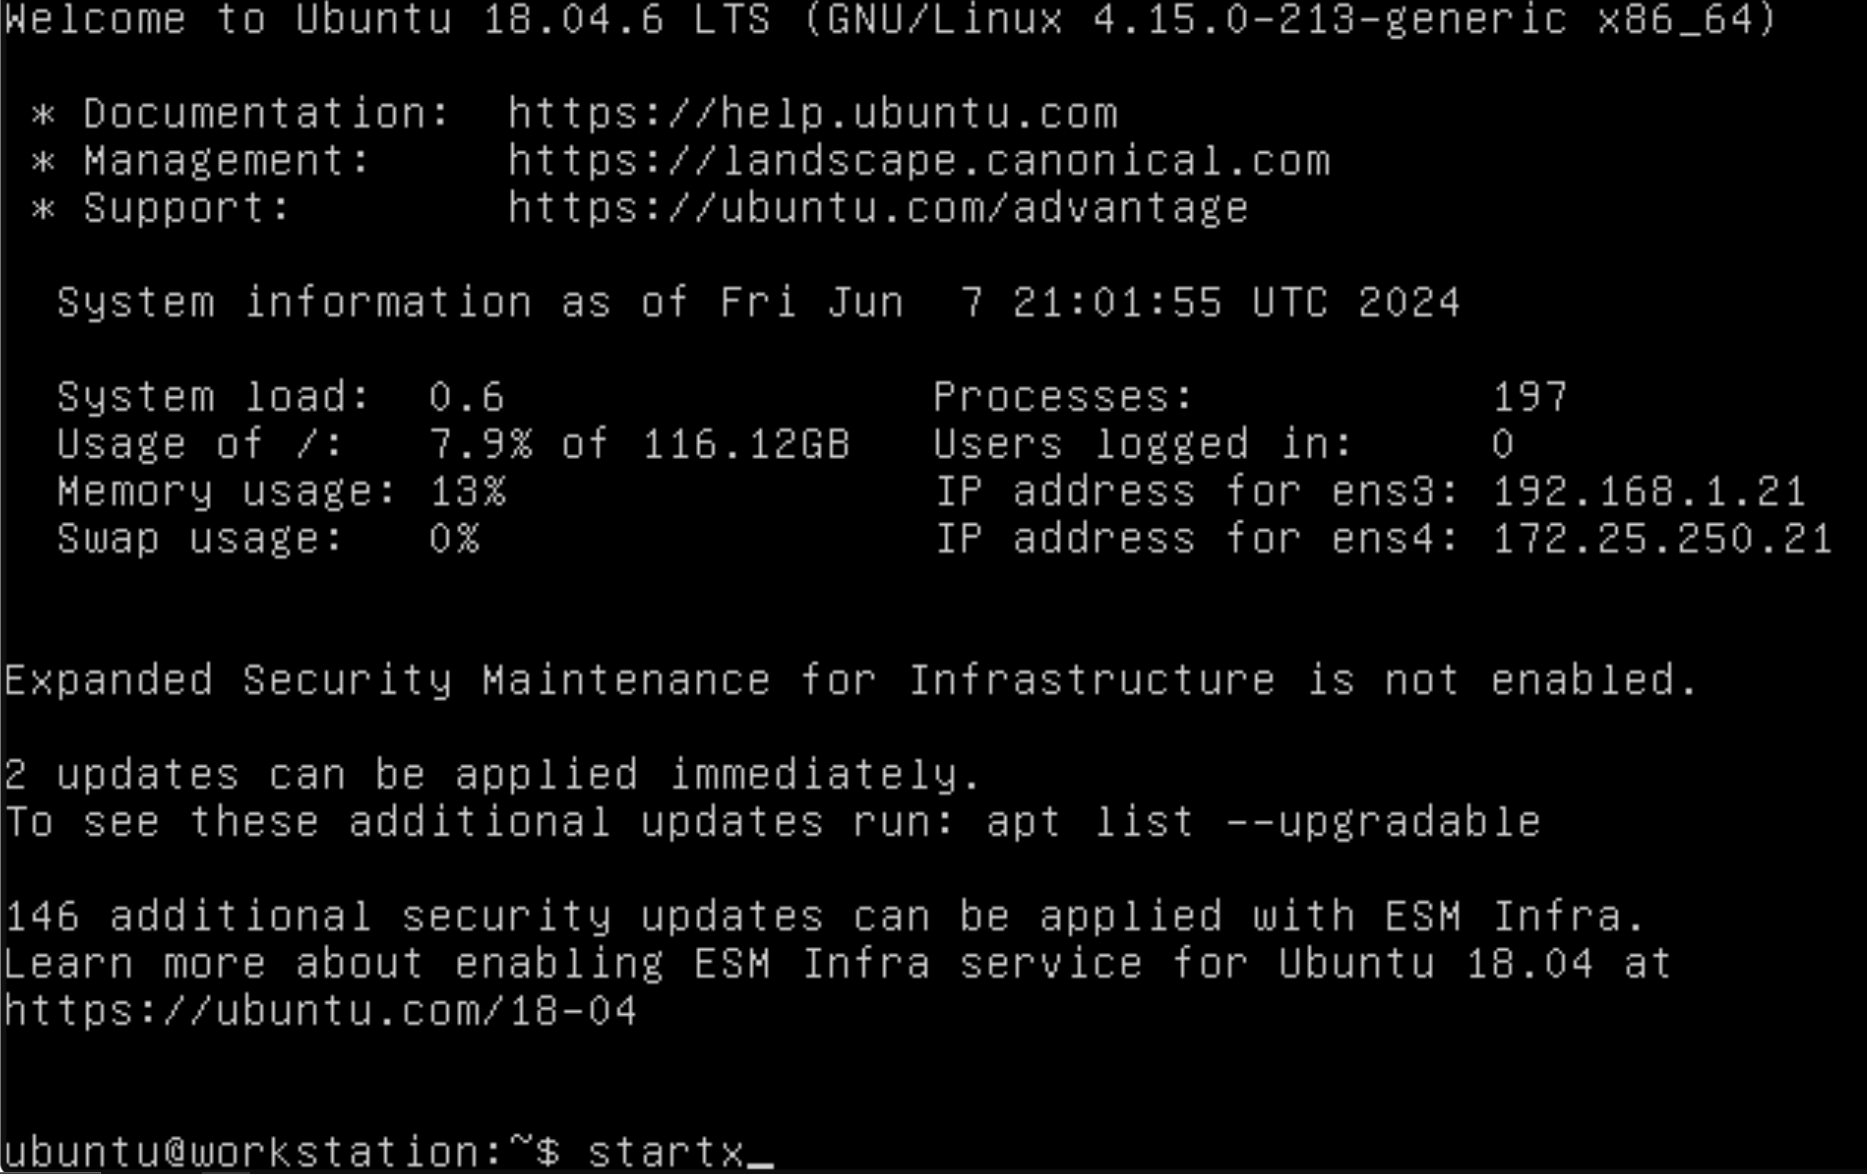
\includegraphics[width=\linewidth]{images/part1/step2.png}
    \end{center}

    \item Open the web browser. Navigate to \textbf{192.168.1.20} and log in to the dashboard as \textbf{admin}
    with the password \textbf{secret}. In this lab, we will create our own public network and router. The \textbf{demo}
    project already has a default router and public network, so those need to be deleted first.

    \item Switch to the \textbf{demo} project. Navigate to \textbf{Admin $>$ Network $>$ Routers}. Check the box in the
    same row as \textbf{router1}, then click \textbf{Delete Routers}.

    \begin{center}
        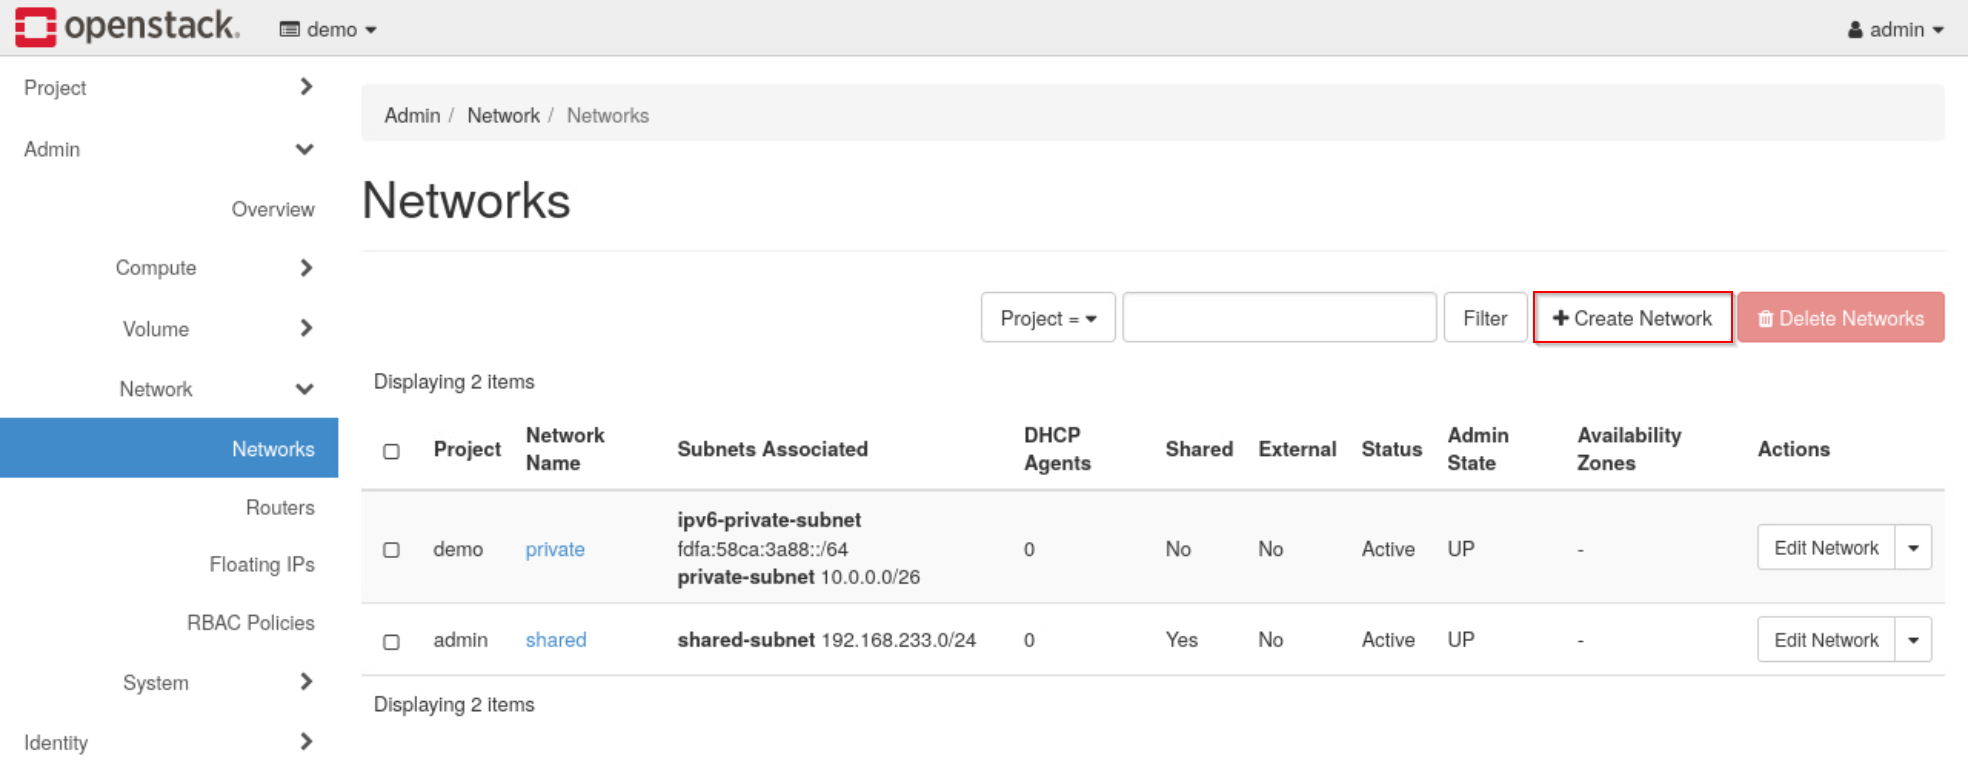
\includegraphics[width=\linewidth]{images/part1/step4.png}
    \end{center}

    \item Now, navigate to \textbf{Networks}. Check the box in the same row as \textbf{public}, then click
    \textbf{Delete Networks}.

    \begin{center}
        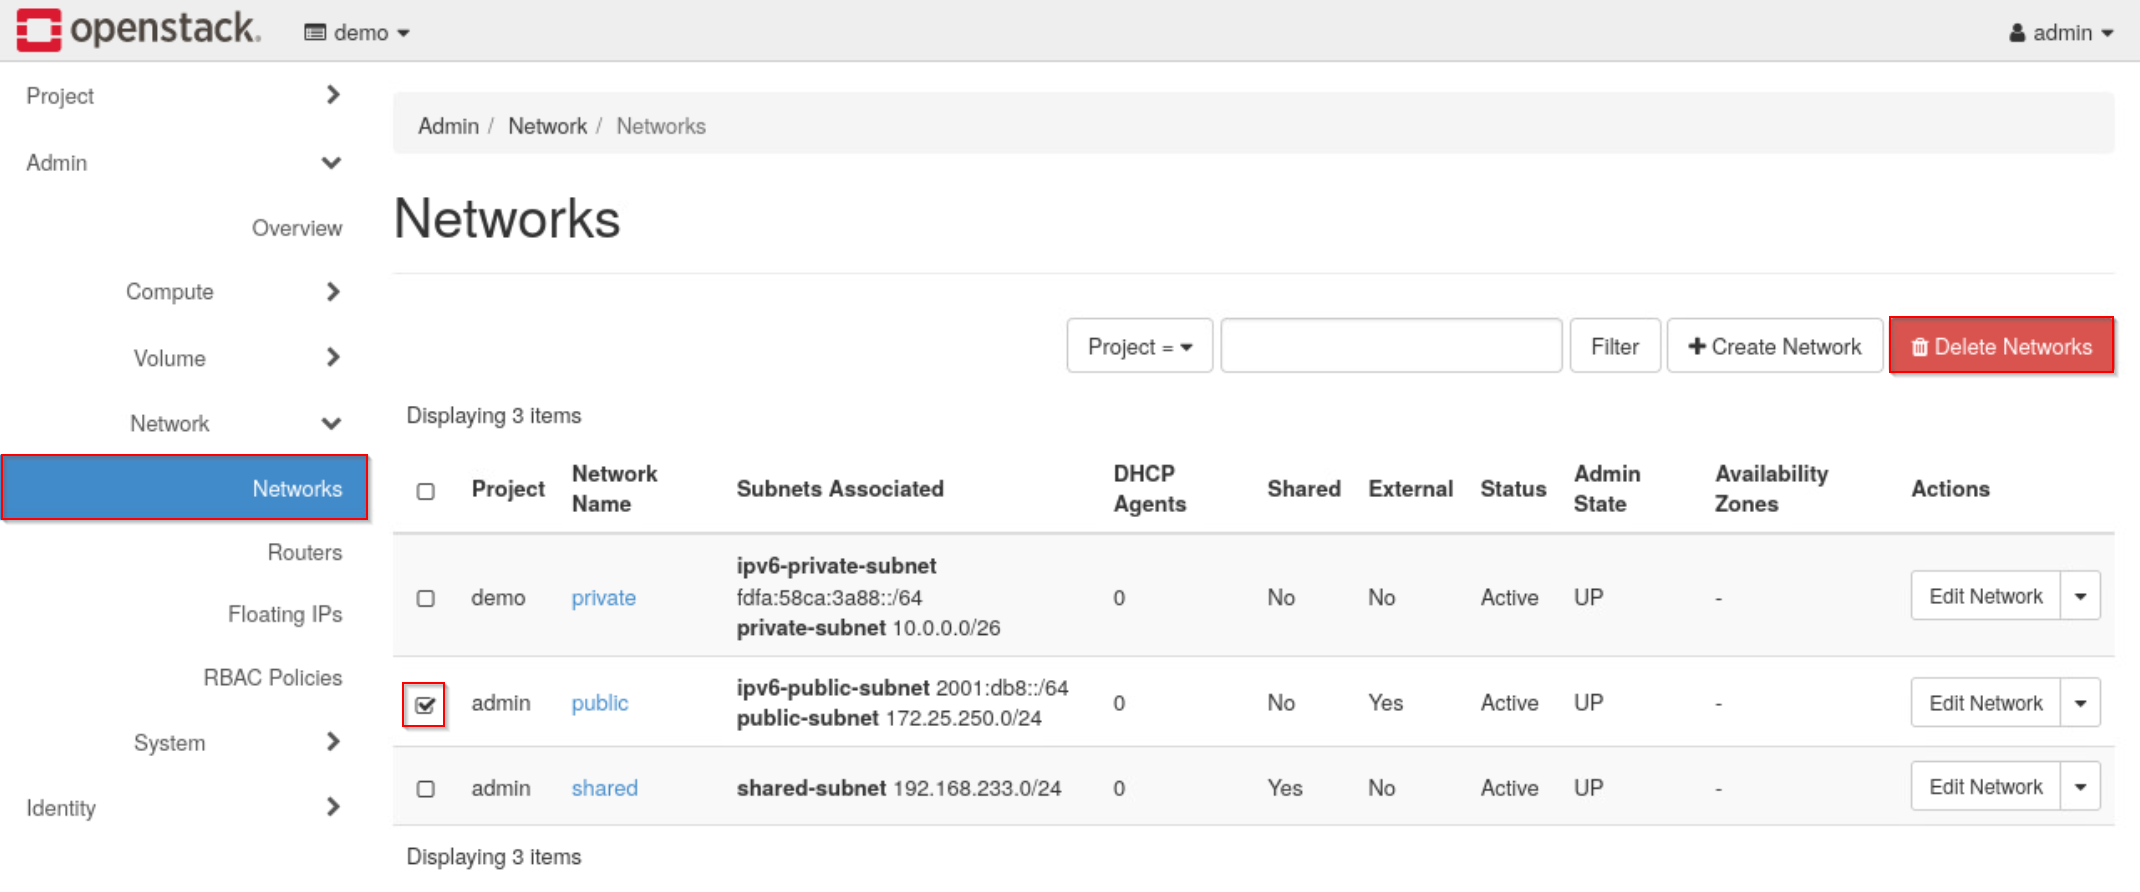
\includegraphics[width=\linewidth]{images/part1/step5.png}
    \end{center}

    \item Click \textbf{Create Network}.
    
    \begin{center}
        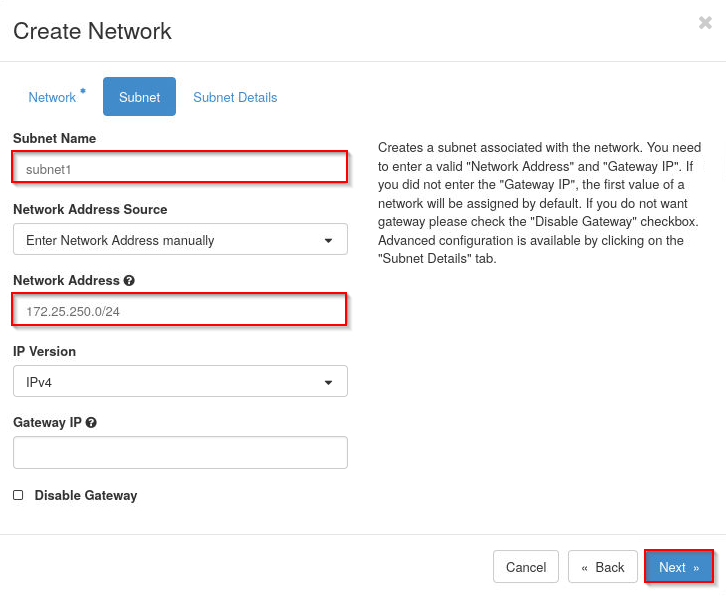
\includegraphics[width=\linewidth]{images/part1/step6.png}
    \end{center}
    
    \item Enter \textbf{extern-net1} in the \textit{Network Name} field. Select \textbf{demo} in the \textit{Project} dropdown.
    For \textit{Provider Network Type}, select \textbf{Flat}. Enter \textbf{public} into the \textit{Physical Network}
    field. Check the \textit{Shared} and \textit{External Network} check boxes, and ensure the \textit{Create Subnet}
    check box is checked. Click \textbf{Next} to go to the \textit{Subnet} tab.

    \begin{center}
        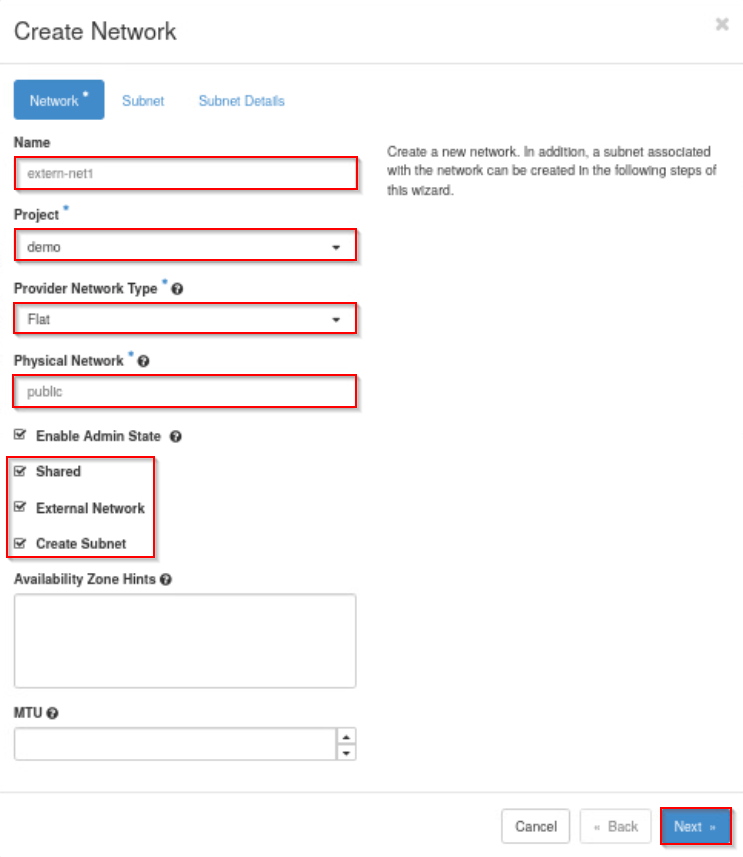
\includegraphics[width=\linewidth]{images/part1/step7.png}
    \end{center}

    \begin{notebox}
        The \textbf{public} physical network is different from the \textbf{public} network we just deleted. This
        physical network is the name assigned to the physical or provider network that OpenStack uses for external
        communication. This resource did not get deleted with the network of the same name since they are independent.
        The \textbf{public} network that was deleted was a virtual network implemented on top of the physical network.
    \end{notebox}

    \item In the \textit{Subnet} tab, enter \textbf{extern-subnet1} in the \textit{Subnet Name} field, enter
    \textbf{172.25.250.0/24} in the \textit{Network Address} field, and enter \textbf{172.25.250.254} in the
    \textit{Gateway IP} field.  Click \textbf{Next} to go to the \textit{Subnet Details} tab.

    \begin{center}
        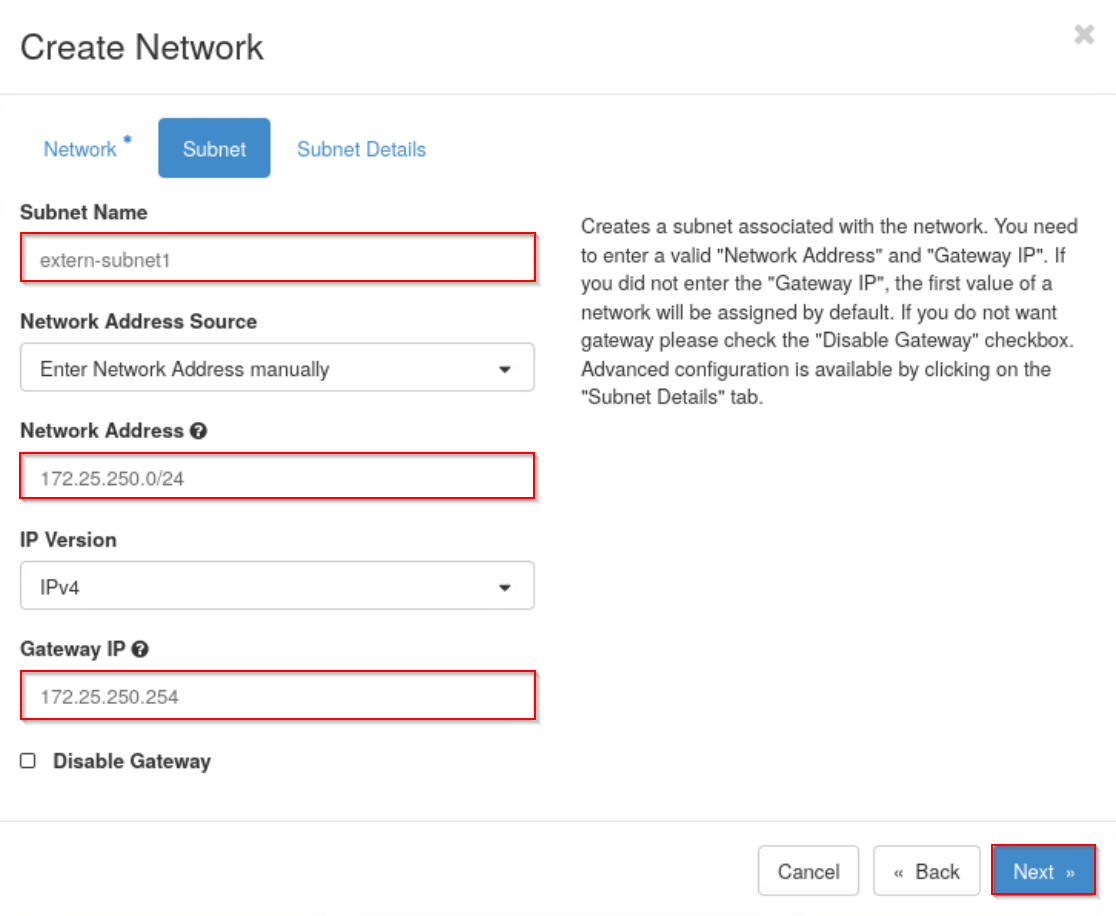
\includegraphics[width=\linewidth]{images/part1/step8.png}
    \end{center}

    \item In the \textit{Subnet Details} tab, uncheck the \textit{Enable DHCP} check box since we want to assign static
    IP addresses on this network. Enter \textbf{172.25.250.60, 172.25.250.80} in the \textit{Allocation Pools} field so
    that any IP address allocated for this network will fall in this range of addresses. Enter \textbf{172.25.250.254}
    in the \textit{DNS Name Servers} field. Click \textbf{Create} to create the network and subnet.

    \begin{center}
        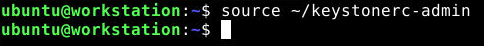
\includegraphics[width=\linewidth]{images/part1/step9.png}
    \end{center}

    \item Log out of the \textit{Horizon Dashboard} and close the web browser.
    
    \item Open a terminal window and source the keystone credentials for the \textbf{admin} user.
    \begin{lstlisting}
        ubuntu@workstation:~$ source ~/keystonerc-admin
    \end{lstlisting}

    \begin{center}
        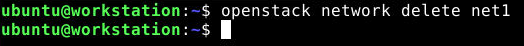
\includegraphics[width=\linewidth]{images/part1/step11.png}
    \end{center}

    \item List the available networks.
    \begin{lstlisting}
        [ubuntu@workstation (keystone-admin)]:~$ openstack network list \
        > --max-width 100
    \end{lstlisting}

    \begin{center}
        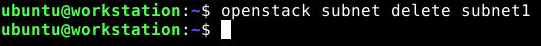
\includegraphics[width=\linewidth]{images/part1/step12.png}
    \end{center}

    \begin{tipbox}
        When typing the command, make sure there is a space between \textbf{extern-net2} and the
        \textbf{\textbackslash} character, and press \textbf{Enter} to get the \textbf{$>$} and continue typing the rest
        of the command.
    \end{tipbox}

    \begin{tipbox}
        To keep the output from overflowing while keeping the formatting intact, use the \textbf{--max-width n} option
        to limit the output to \textbf{n} characters per line. This is especially useful for commands that output long
        IDs or have many columns in the output table.
    \end{tipbox}

    \item The next set of steps will show how to recreate the external network from the beginning of the lab using the
    CLI. To free up the necessary resources, first delete the \textbf{extern-net1} network. This will also delete the
    \textbf{extern-subnet1} subnet.
    \begin{lstlisting}
        [ubuntu@workstation (keystone-admin)]:~$ openstack network delete extern-net1
    \end{lstlisting}

    \begin{center}
        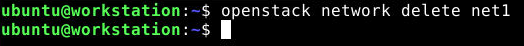
\includegraphics[width=\linewidth]{images/part1/step13.png}
    \end{center}

    \item List the networks again to confirm that \textbf{extern-net1} was deleted successfully.
    \begin{lstlisting}
        [ubuntu@workstation (keystone-admin)]:~$ openstack network list \
        > --max-width 100
    \end{lstlisting}

    \begin{center}
        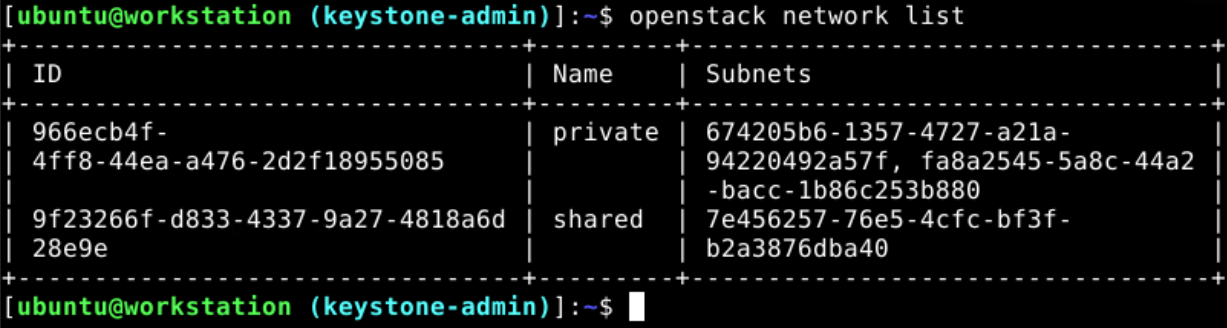
\includegraphics[width=\linewidth]{images/part1/step14.png}
    \end{center}

    \item Create an external network named \textbf{extern-net2}. Set the network type to \textbf{flat} and the physical
    network to \textbf{public}. Set the network as shared and external.
    \begin{lstlisting}
        [ubuntu@workstation (keystone-admin)]:~$ openstack network create \
        > --external --share \
        > --provider-network-type flat \
        > --provider-physical-network public \
        > extern-net2
    \end{lstlisting}

    \begin{center}
        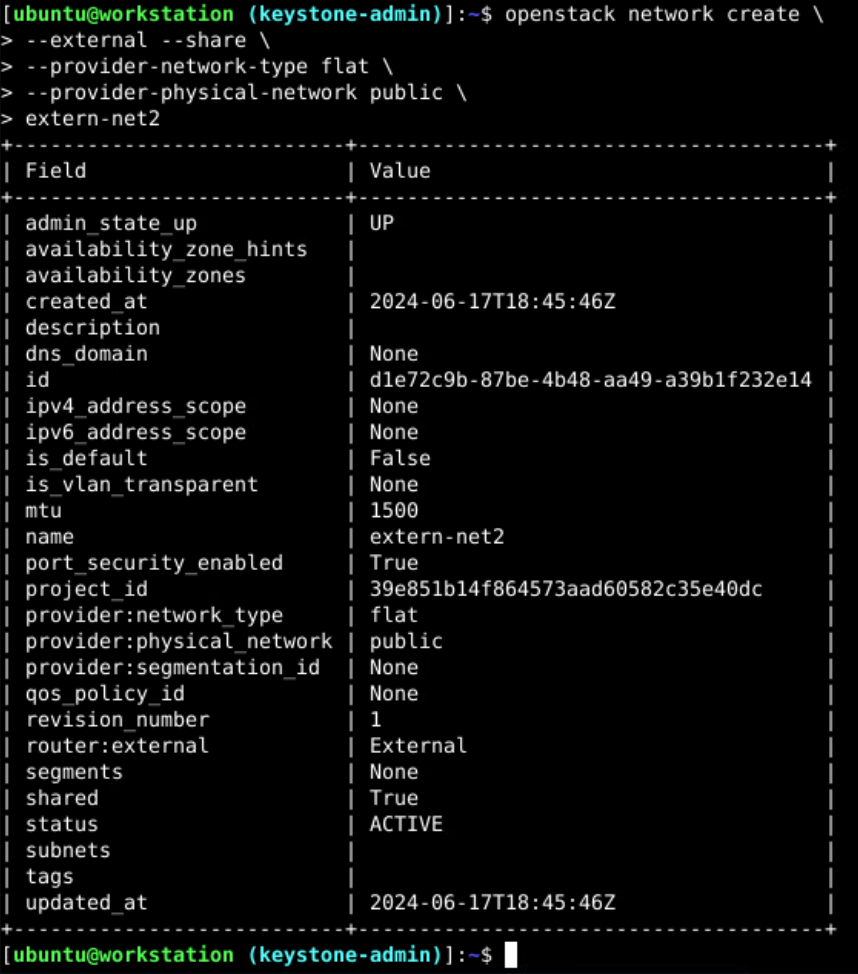
\includegraphics[width=\linewidth]{images/part1/step15.png}
    \end{center}

    \item Create a subnet named \textbf{extern-subnet2} in the \textbf{extern-net2} network. Give the subnet a range of
    \textbf{172.25.250.60} to \textbf{172.25.250.80}. Disable DHCP services for the subnet and use the address
    \textbf{172.25.250.254} as the gateway as well as the DNS name server.
    \begin{lstlisting}
        [ubuntu@workstation (keystone-admin)]:~$ openstack subnet create \
        > --subnet-range 172.25.250.0/24 \
        > --no-dhcp \
        > --gateway 172.25.250.254 \
        > --dns-nameserver 172.25.250.254 \
        > --allocation-pool start=172.25.250.60,end=172.25.250.80 \
        > --network extern-net2 \
        > extern-subnet2
    \end{lstlisting}

    \begin{center}
        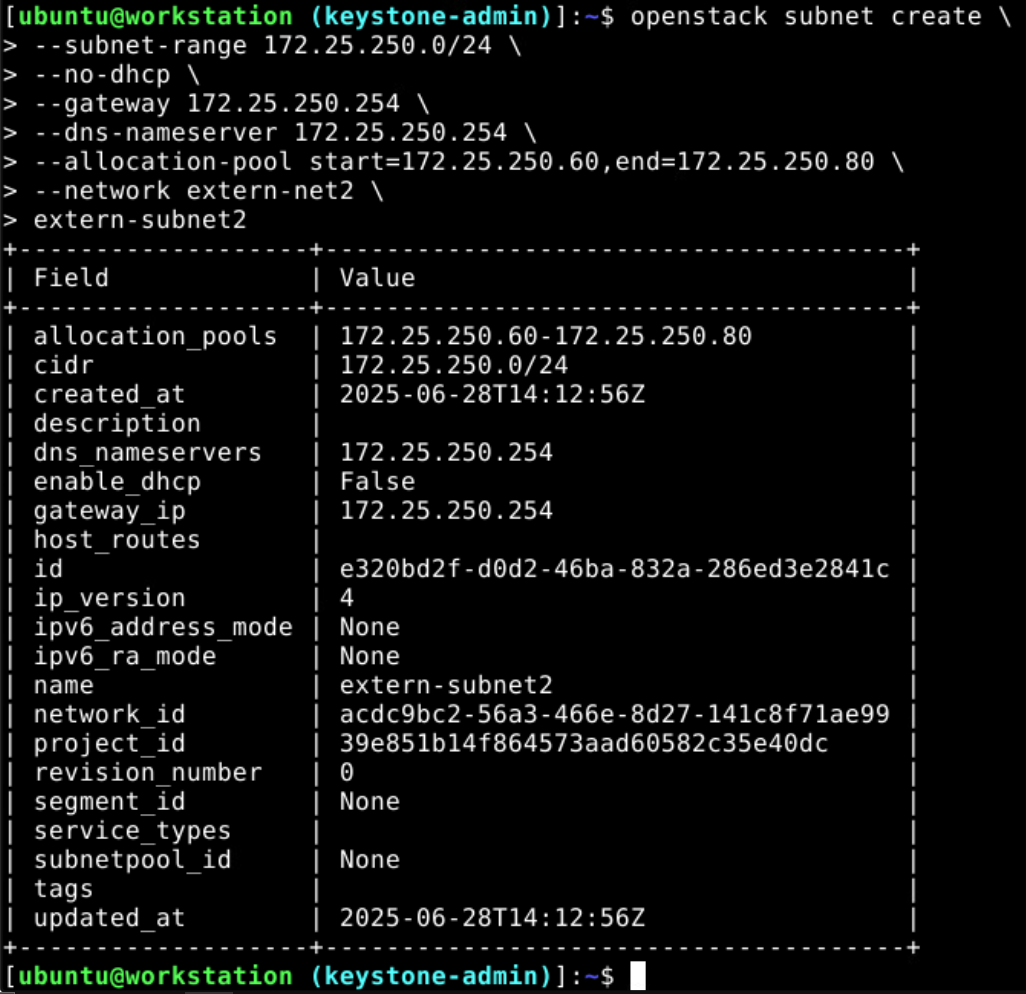
\includegraphics[width=\linewidth]{images/part1/step16.png}
    \end{center}

    \item List the networks again to see that \textbf{extern-net2} and \textbf{extern-subnet2} were created
    successfully.
    \begin{lstlisting}
        [ubuntu@workstation (keystone-admin)]:~$ openstack network list \
        > --max-width 100
    \end{lstlisting}

    \begin{center}
        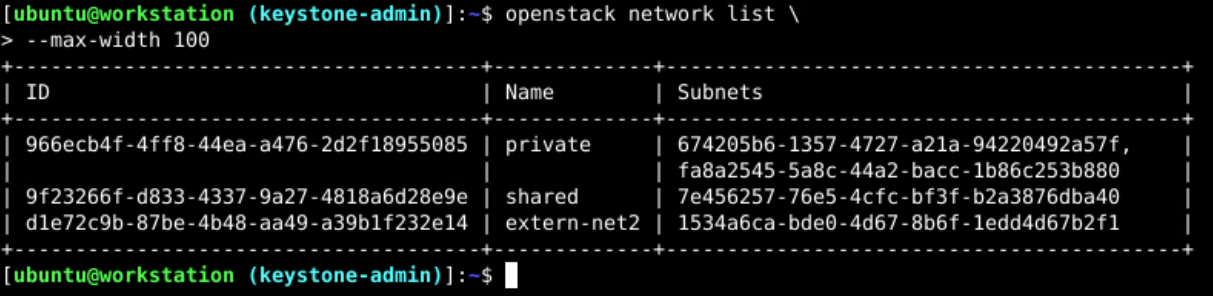
\includegraphics[width=\linewidth]{images/part1/step17.png}
    \end{center}

    \item Leave the terminal window open and continue to the next task.

\end{enumerate}

%%%%%%%%%%%
% Section 2
%%%%%%%%%%%
\section{Preparing OpenStack Routers to Deploy an Instance}
\label{sec:preparing_openstack_routers_to_deploy_an_instance}
In this task, you will create and configure a router using the \textit{Horizon Dashboard} and \textit{OpenStack Unified
CLI} and use command line tools to test the connectivity of the router. The router will serve to connect the external
instance to other networks both within OpenStack and outside the cloud.

\begin{enumerate}
    \item Open the web browser and navigate to \textbf{192.168.1.20}. Log into the dashboard as \textbf{admin} with the
    password \textbf{secret}.

    \item Switch to the \textbf{demo} project and navigate to \textbf{Project $>$ Network $>$ Routers}. Click
    \textbf{Create Router} to create a new router.
    
    \begin{center}
        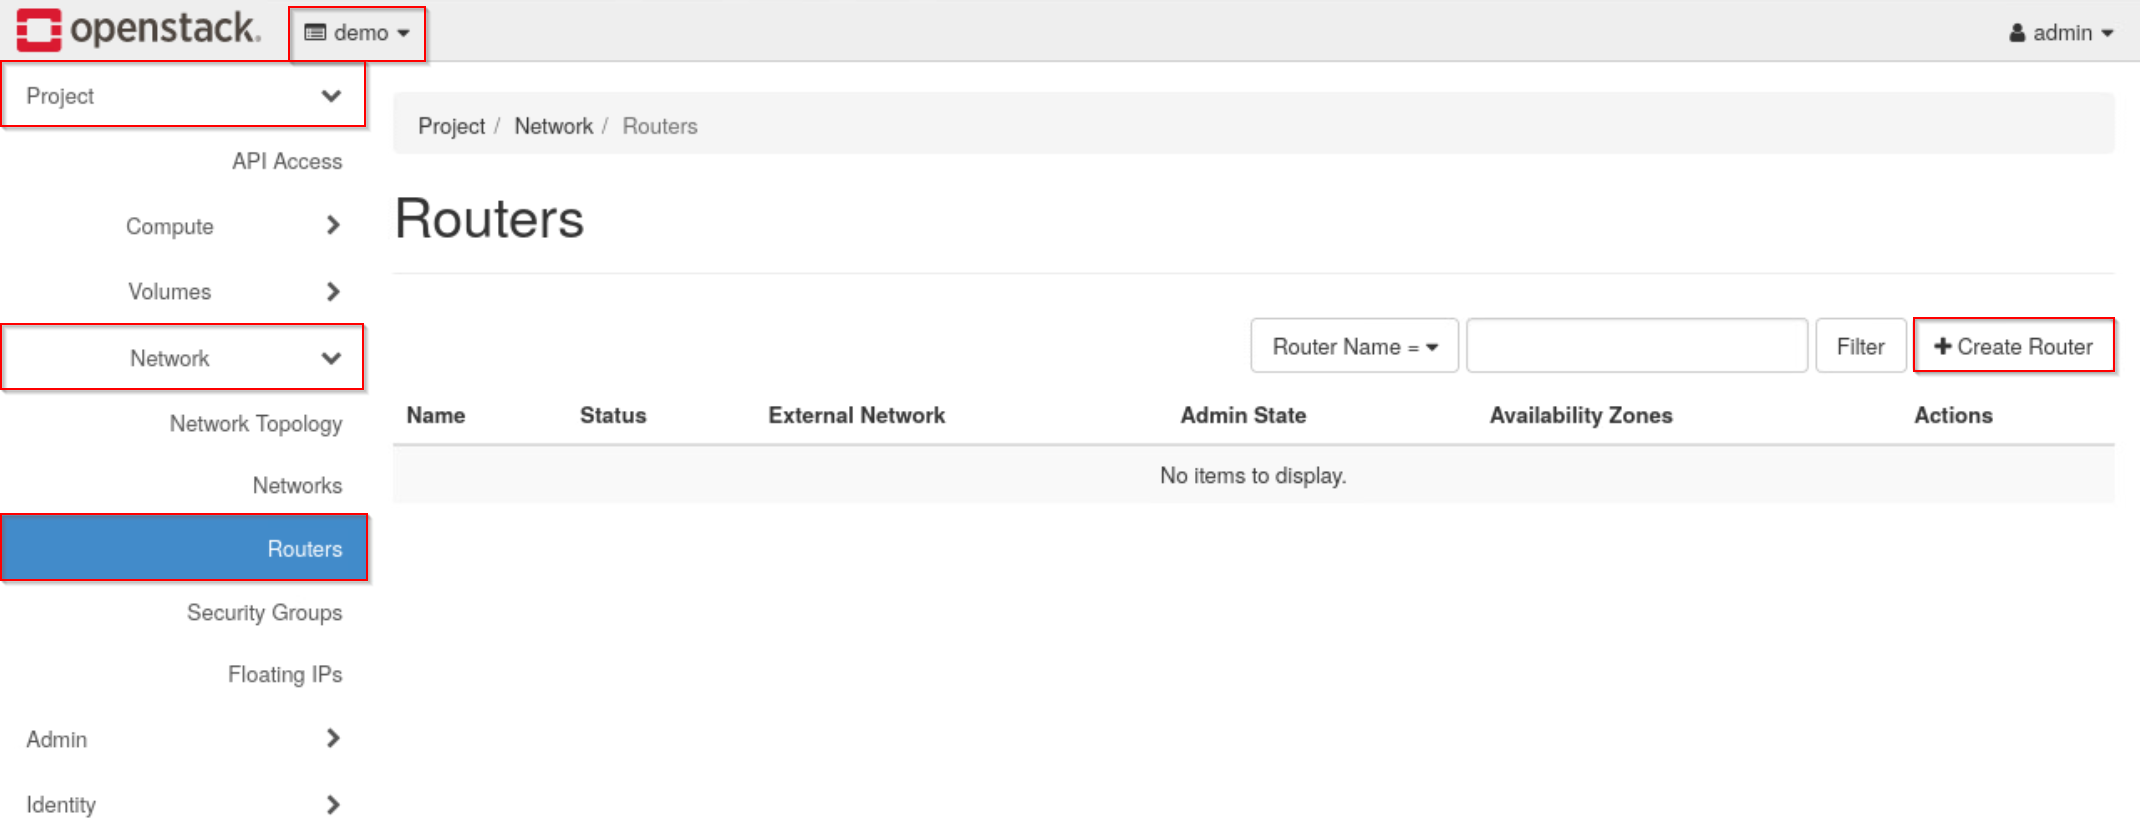
\includegraphics[width=\linewidth]{images/part2/step2.png}
    \end{center}

    \item Enter \textbf{router1} in the \textit{Router Name} field and select \textbf{extern-net2} in the
    \textit{External Network} dropdown. Click \textbf{Create Router}.

    \begin{center}
        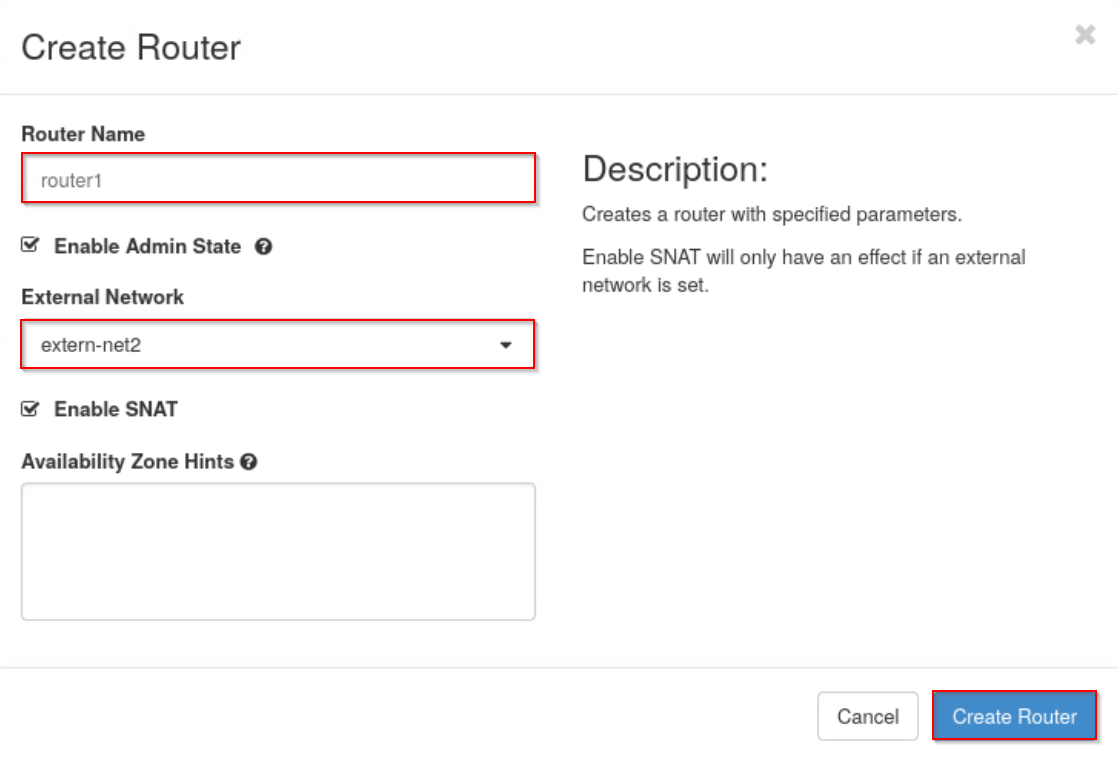
\includegraphics[width=\linewidth]{images/part2/step3.png}
    \end{center}

    \item Click the router name, \textbf{router1}, to access its details.
    
    \begin{center}
        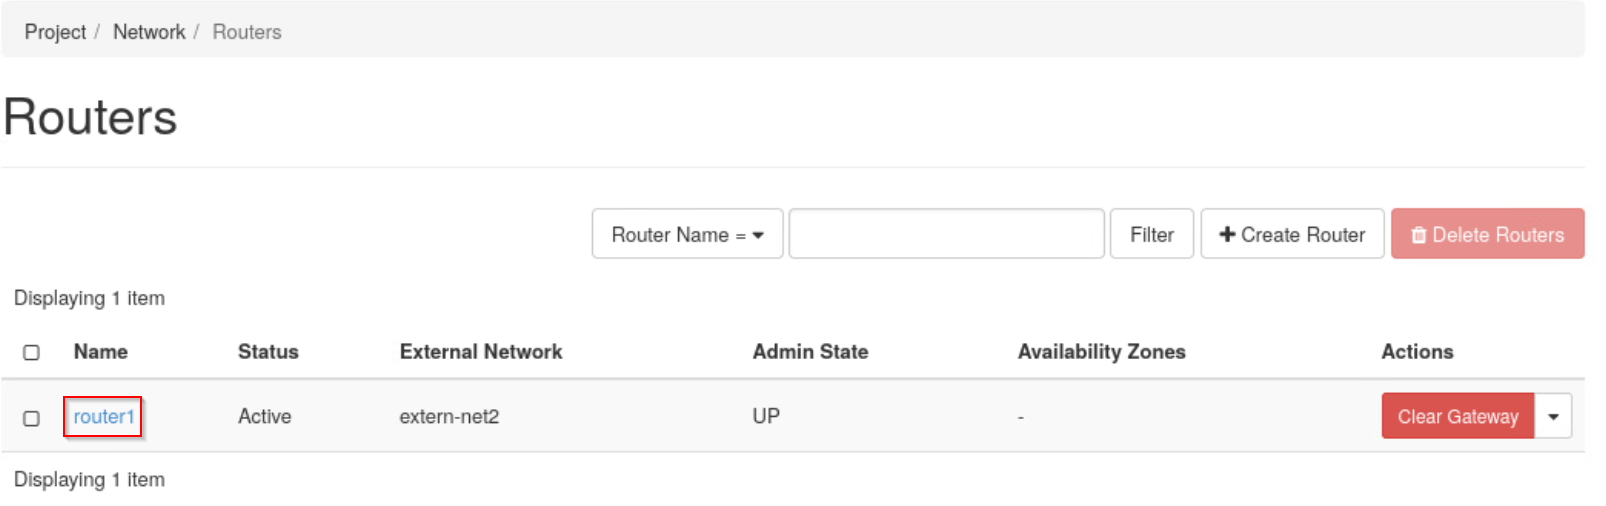
\includegraphics[width=\linewidth]{images/part2/step4.png}
    \end{center}

    \item Click the \textbf{Interfaces} tab to manage the interfaces for the router. Notice that currently, the router
    only has an interface connecting it to the \textbf{extern-net2} external network. This will connect instances on
    this network to networks outside the cloud. We will add an interface to connect \textbf{extern-net2} to another
    network within the OpenStack cloud environment. Click \textbf{Add Interface} to add a new interface.

    \begin{center}
        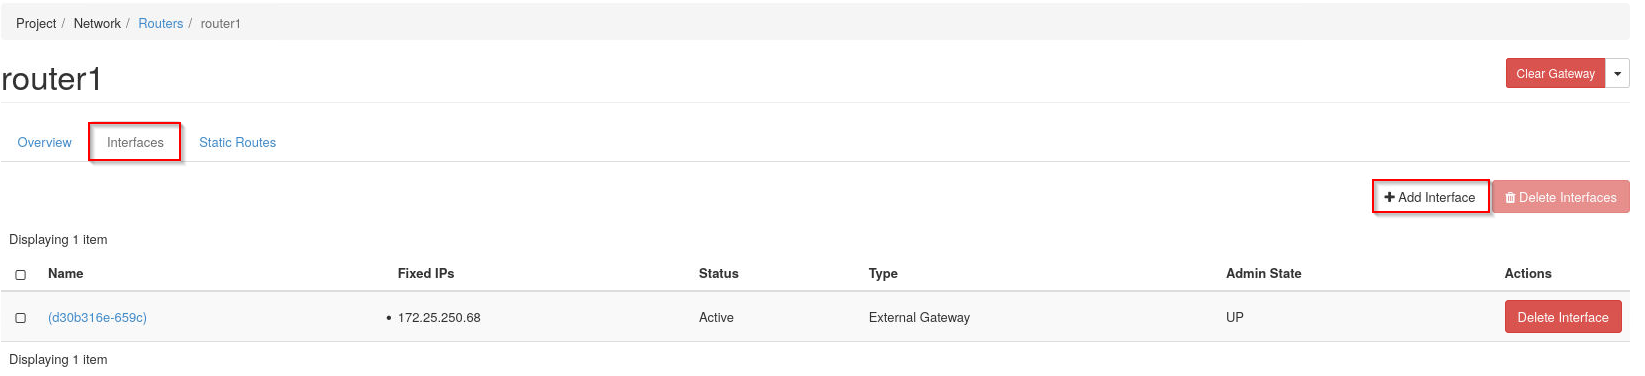
\includegraphics[width=\linewidth]{images/part2/step5.png}
    \end{center}

    \item Select \textbf{shared: 172.25.233.0/24 (shared-subnet)} from the \textit{Subnet} dropdown and click
    \textbf{Submit} to add the interface. This will connect the \textbf{extern-net2} network to the \textbf{shared}
    network.

    \begin{center}
        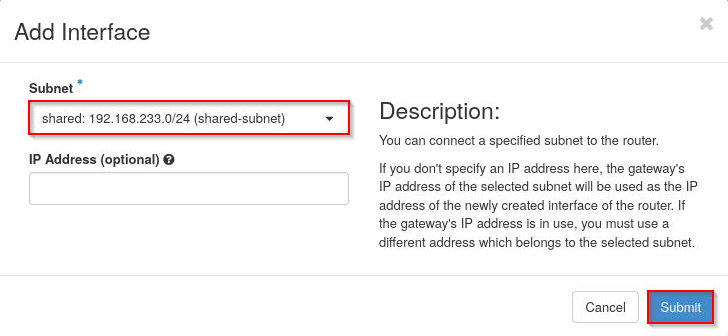
\includegraphics[width=\linewidth]{images/part2/step6.png}
    \end{center}

    \begin{tipbox}
        You can delete an interface by selecting the checkbox next to the interface name, then clicking \textbf{Delete
        Interfaces}. Alternatively, simply click \textbf{Delete Interface} in the same row as the target interface.
    \end{tipbox}

    \item Log out of the dashboard and close the web browser.
    
    \item Open a terminal window if one is not already open, and source the \textbf{admin} credentials.
    \begin{lstlisting}
        ubuntu@workstation:~$ source ~/keystonerc-admin
    \end{lstlisting}

    \begin{center}
        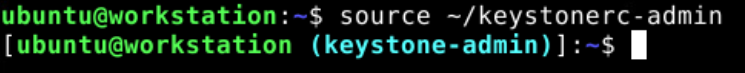
\includegraphics[width=\linewidth]{images/part2/step8.png}
    \end{center}

    \item Next, we will recreate this router using the CLI, so we will delete \textbf{router1}. First, however, we will
    see how to remove subnets and gateways from the router. Recall that in a previous step, we added an interface to
    connect \textbf{router1} to the the \textbf{shared-subnet} subnet on the \textbf{shared} network. Remove the
    connection to this subnet.
    \begin{lstlisting}
        [ubuntu@workstation (keystone-admin)]:~$ openstack router remove subnet \
        > router1 \
        > shared-subnet
    \end{lstlisting}

    \begin{center}
        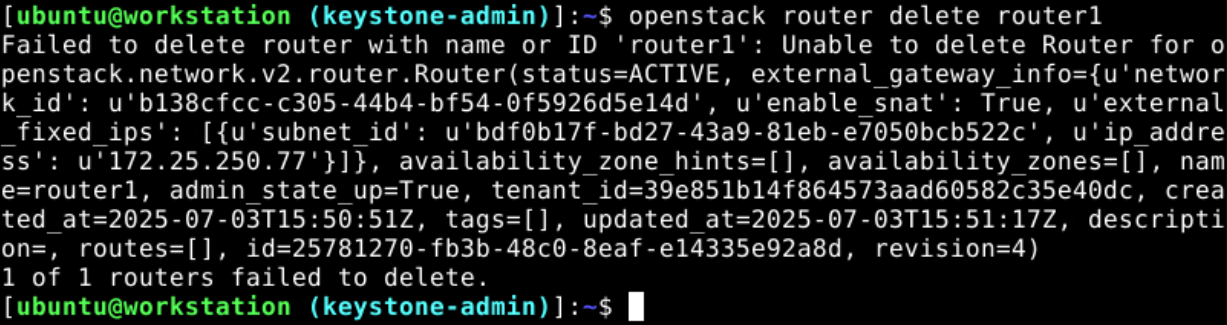
\includegraphics[width=\linewidth]{images/part2/step9.png}
    \end{center}

    \item Unset the \textbf{extern-net2} network as the gateway for the router.
    \begin{lstlisting}
        [ubuntu@workstation (keystone-admin)]:~$ openstack router unset \
        > --external-gateway router2
    \end{lstlisting}

    \begin{center}
        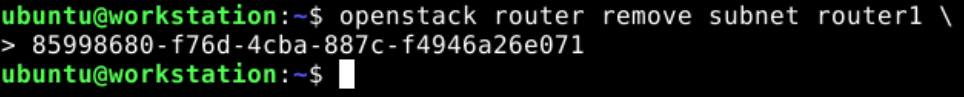
\includegraphics[width=\linewidth]{images/part2/step10.png}
    \end{center}

    \item Delete the \textbf{router1} router.
    \begin{lstlisting}
        [ubuntu@workstation (keystone-admin)]:~$ openstack router delete router1
    \end{lstlisting}

    \begin{center}
        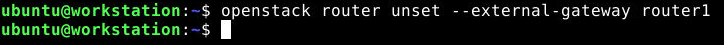
\includegraphics[width=\linewidth]{images/part2/step11.png}
    \end{center}

    \begin{notebox}
        Deleting a router will also delete its associated interfaces, subnets, and gateways. The previous steps that
        performed these steps manually were only for demonstration and are not necessary for simply deleting the router.
    \end{notebox}

    \item Now, we will replicate the previous router using the CLI. Create a router named \textbf{router2}.
    \begin{lstlisting}
        [ubuntu@workstation (keystone-admin)]:~$ openstack router create router2
    \end{lstlisting}

    \begin{center}
        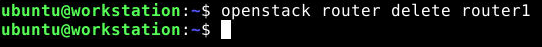
\includegraphics[width=\linewidth]{images/part2/step12.png}
    \end{center}

    \item Connect the router to the \textbf{shared-subnet} subnet.
    \begin{lstlisting}
        [ubuntu@workstation (keystone-admin)]:~$ openstack router add subnet \
        > router2 \
        > shared-subnet
    \end{lstlisting}

    \begin{center}
        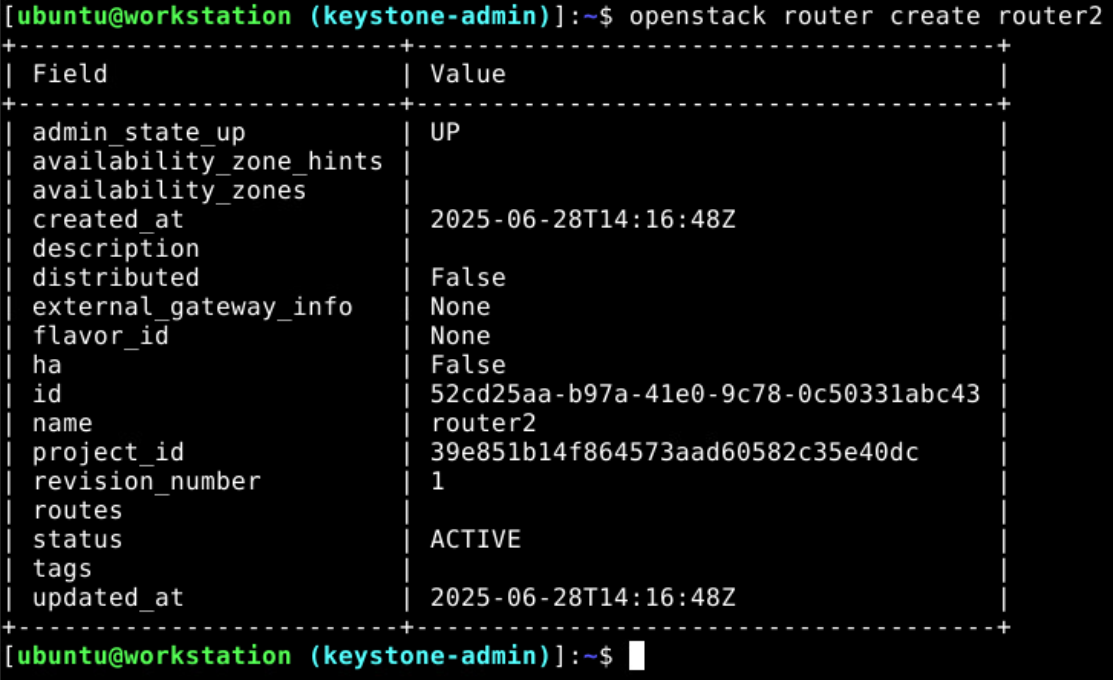
\includegraphics[width=\linewidth]{images/part2/step13.png}
    \end{center}

    \item Set the \textbf{extern-net2} network as the gateway for the router.
    \begin{lstlisting}
        [ubuntu@workstation (keystone-admin)]:~$ openstack router set \
        > --external-gateway extern-net2 \
        > router2
    \end{lstlisting}

    \begin{center}
        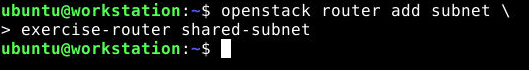
\includegraphics[width=\linewidth]{images/part2/step14.png}
    \end{center}

    \item Show the details of the \textbf{router2} router. Take note of the IP address listed in the
    \textit{external\_gateway\_info} row, as you will ping this address in a later step to verify that the router can be
    reached.
    \begin{lstlisting}
        [ubuntu@workstation (keystone-admin)]:~$ openstack router show \
        > --max-width 100 router2
    \end{lstlisting}

    \begin{center}
        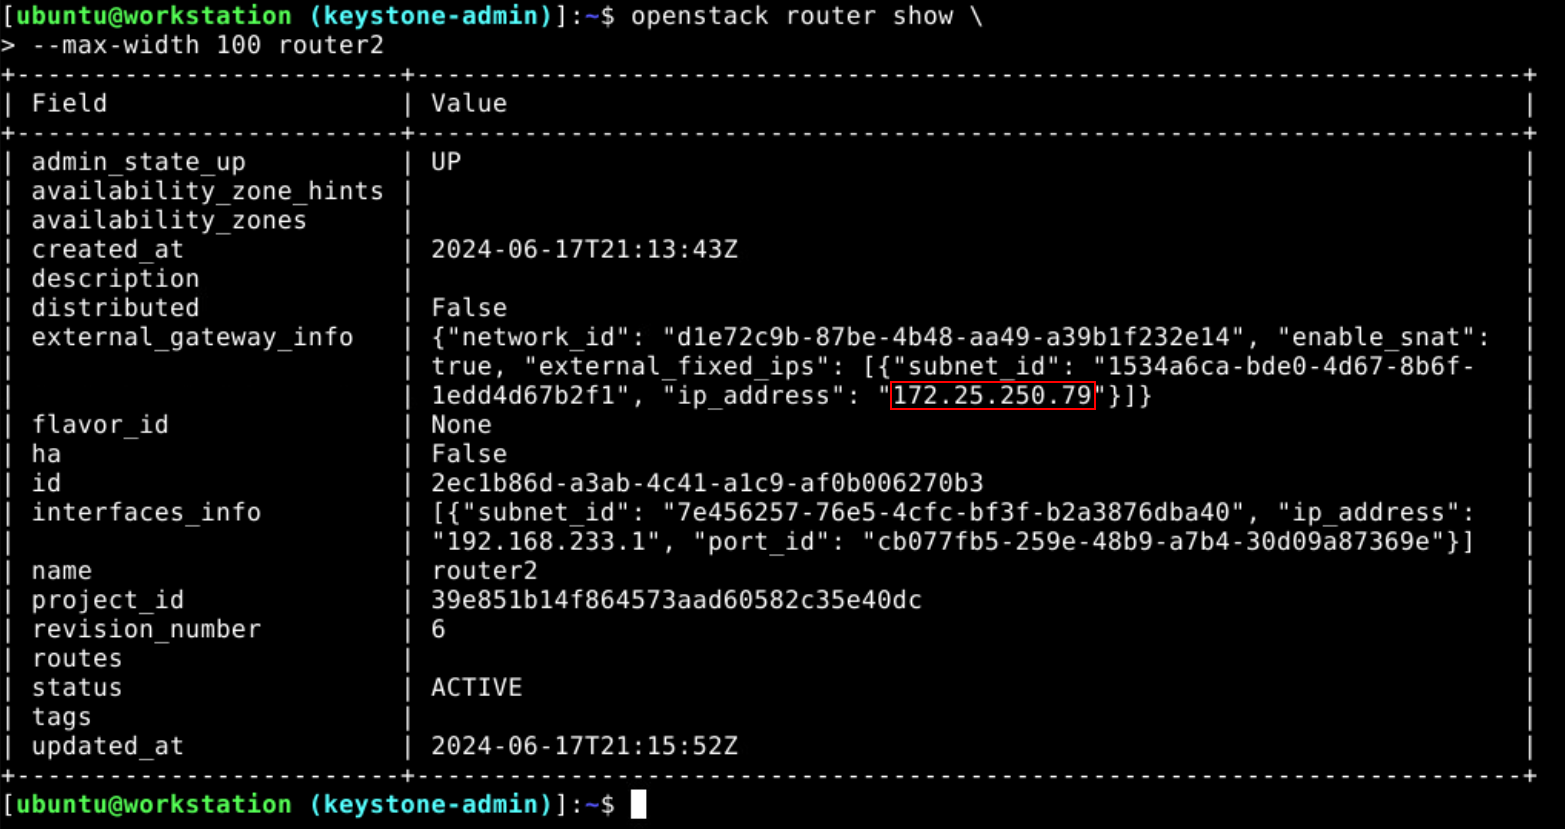
\includegraphics[width=\linewidth]{images/part2/step15.png}
    \end{center}

    \item In order to test the connectivity of the router, SSH into the \textbf{devstack} virtual machine. Log in with
    the password \textbf{ubuntu}.
    \begin{lstlisting}
        [ubuntu@workstation (keystone-admin)]:~$ ssh 192.168.1.20
    \end{lstlisting}

    \begin{center}
        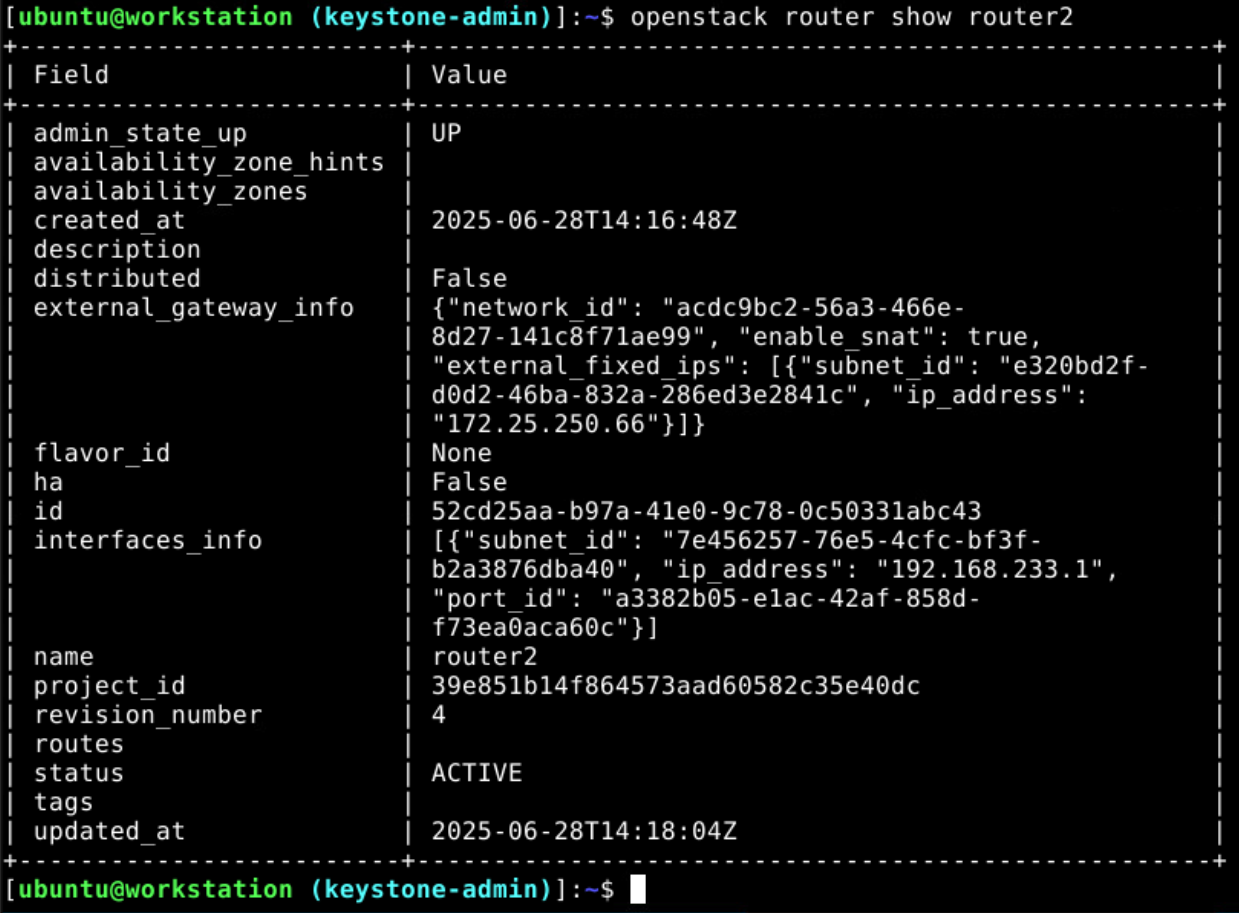
\includegraphics[width=\linewidth]{images/part2/step16.png}
    \end{center}

    \item Use the \textbf{ping} command on the IP address found from the \textbf{openstack router show} command to
    verify that the router can be reached. Receiving ping replies verifies the connectivity of the router since the
    \textbf{devstack} machine is outside of the OpenStack cloud environment.
    \begin{lstlisting}
        ubuntu@devstack:~$ ping -c3 172.25.250.79
    \end{lstlisting}

    \begin{center}
        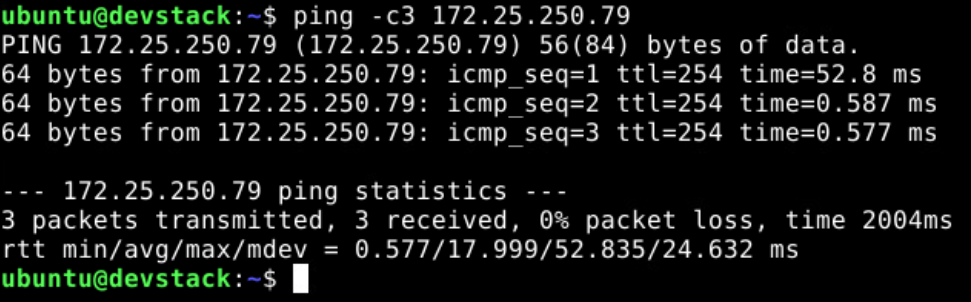
\includegraphics[width=\linewidth]{images/part2/step17.png}
    \end{center}

    \begin{notebox}
        The actual IP address may differ from this example.
    \end{notebox}
    \begin{notebox}
        You should receive three successful ping replies.
    \end{notebox}

    \item Exit the SSH session.
    \begin{lstlisting}
        [ubuntu@workstation (keystone-admin)]:~$ exit
    \end{lstlisting}

    \begin{center}
        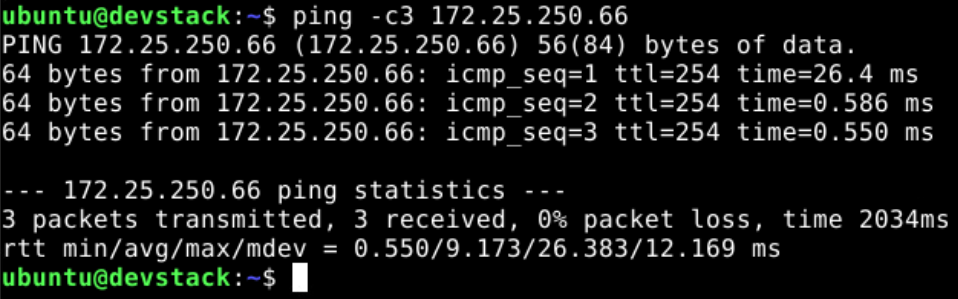
\includegraphics[width=\linewidth]{images/part2/step18.png}
    \end{center}

    \item Leave the terminal window open and continue to the next task.

\end{enumerate}

%%%%%%%%%%%
% Section 3
%%%%%%%%%%%
\section{Maintaining Floating IP Addresses}
\label{sec:maintaining_floating_ip_addresses}
In this task, you will create a floating IP address and allocate it to an instance using the Horizon Dashboard and the
OpenStack Unified CLI. While instances are assigned a private, fixed IP address at creation to communicate with other
instances, they can also be assigned a floating IP address, which is used for communication outside of the OpenStack
cloud environment. While the private IP address of instance is fixed until the instance is deleted, a floating IP
address can be exchanged for a different one while the instance is still running.

\begin{enumerate}
    \item If a terminal window is not already open, open one and source the admin credentials from the 
    \textbf{\texttildemid/keystonerc-admin} file.
    \begin{lstlisting}
        ubuntu@workstation:~$ source ~/keystonerc-admin
    \end{lstlisting}

    \begin{center}
        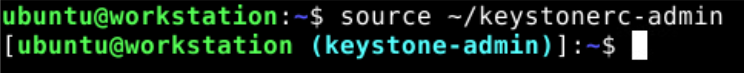
\includegraphics[width=\linewidth]{images/part3/step1.png}
    \end{center}

    \item Create a new instance named \textbf{instance1}. Use the \textbf{ubuntu} image, \textbf{m1.small} flavor, and
    \textbf{shared} network.
    \begin{lstlisting}
        [ubuntu@workstation (keystone-admin)]:~$ openstack server create \
        > --image ubuntu \
        > --flavor m1.small \
        > --nic net-id=shared \
        > instance1
    \end{lstlisting}

    \begin{center}
        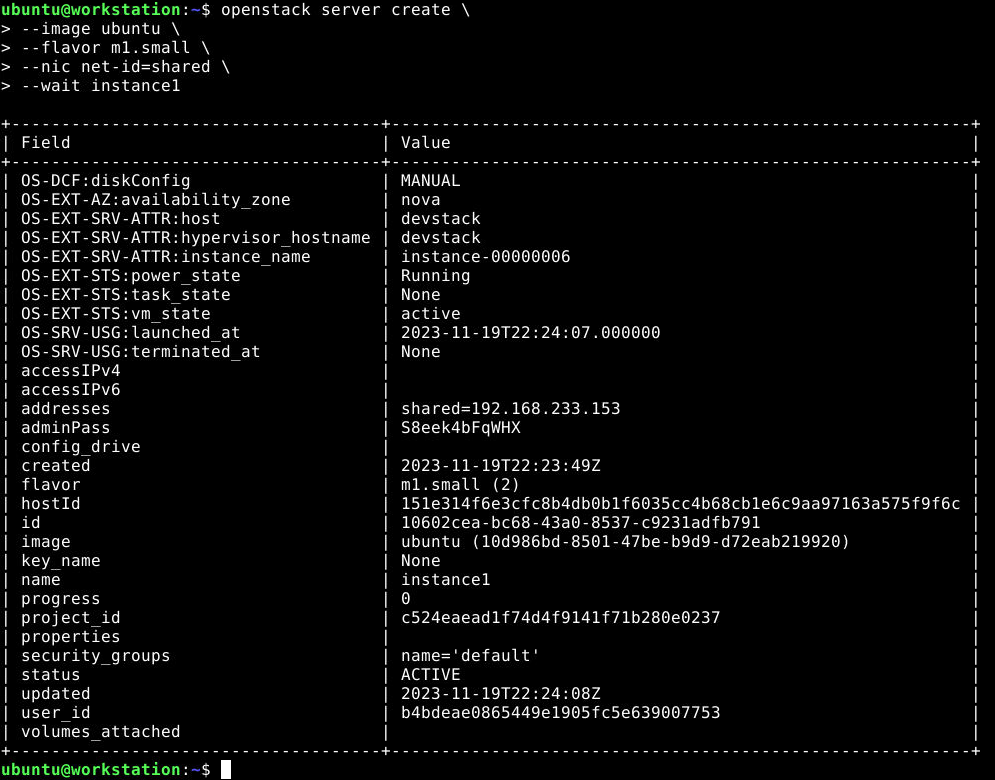
\includegraphics[width=\linewidth]{images/part3/step2.png}
    \end{center}

    \item Leave the terminal window open and open the web browser. Navigate to \textbf{192.168.1.20}. Log into the
    \textit{Horizon Dashboard} as the \textbf{admin} user with the password \textbf{secret}.


    \item Switch to the \textbf{demo} project. Navigate to \textbf{Project $>$ Network $>$ Floating IPs}. Click
    \textbf{Allocate IP to Project}.

    \begin{center}
        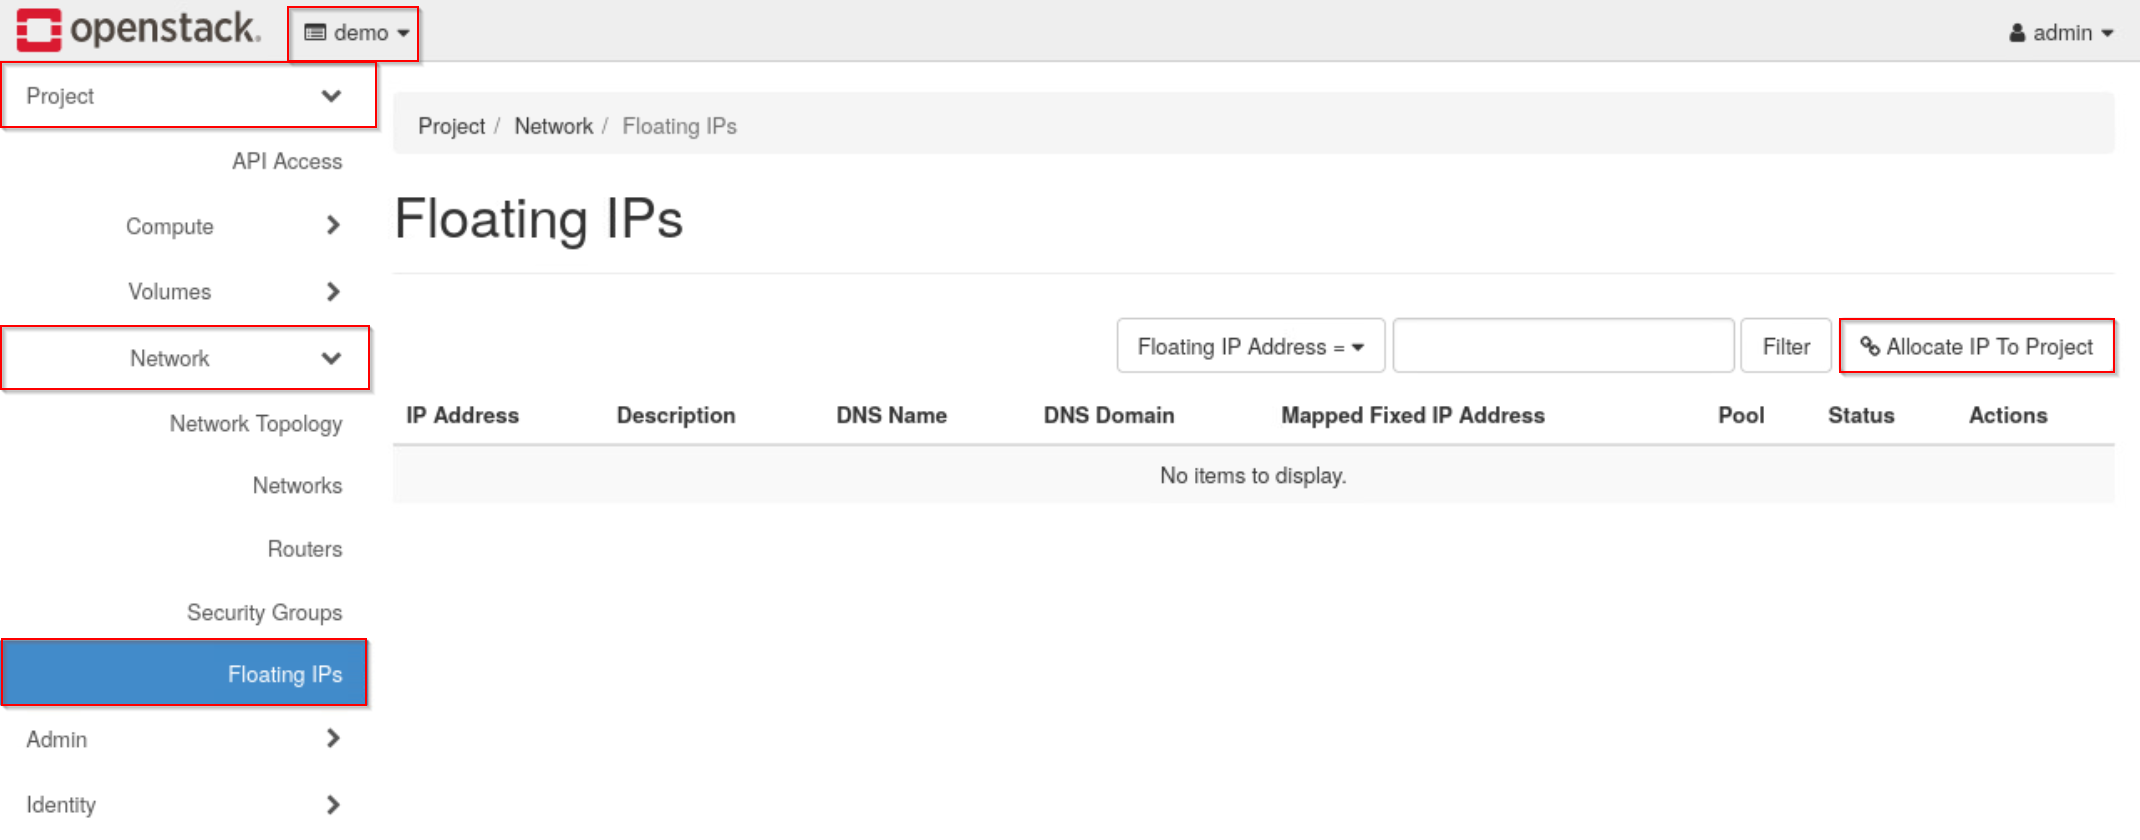
\includegraphics[width=\linewidth]{images/part3/step4.png}
    \end{center}

    \item Ensure \textbf{extern-net2} is set as the \textit{Pool}. Click \textbf{Allocate IP}.
    
    \begin{center}
        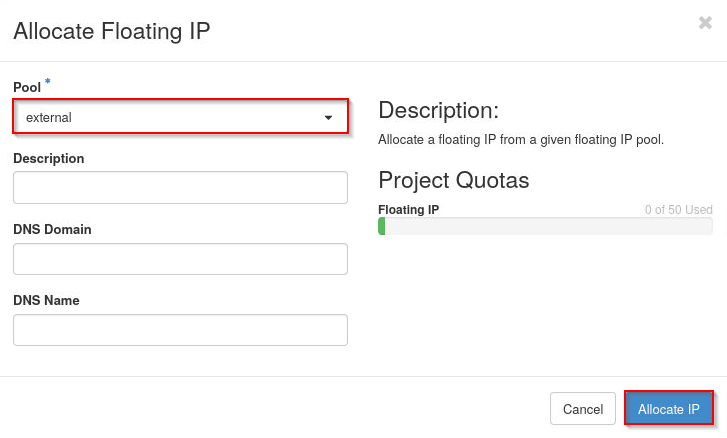
\includegraphics[width=\linewidth]{images/part3/step5.png}
    \end{center}

    \begin{tipbox}
        A floating IP address can be deleted, or released, either by selecting the checkbox next to the floating IP
        address and clicking \textbf{Release Floating IPs}, or by opening the dropdown next to the \textbf{Associate}
        button in the same row as the floating IP address, then clicking \textbf{Release Floating IP}.
    \end{tipbox}

    \item Click \textbf{Associate} in the row of the floating IP address.

    \begin{center}
        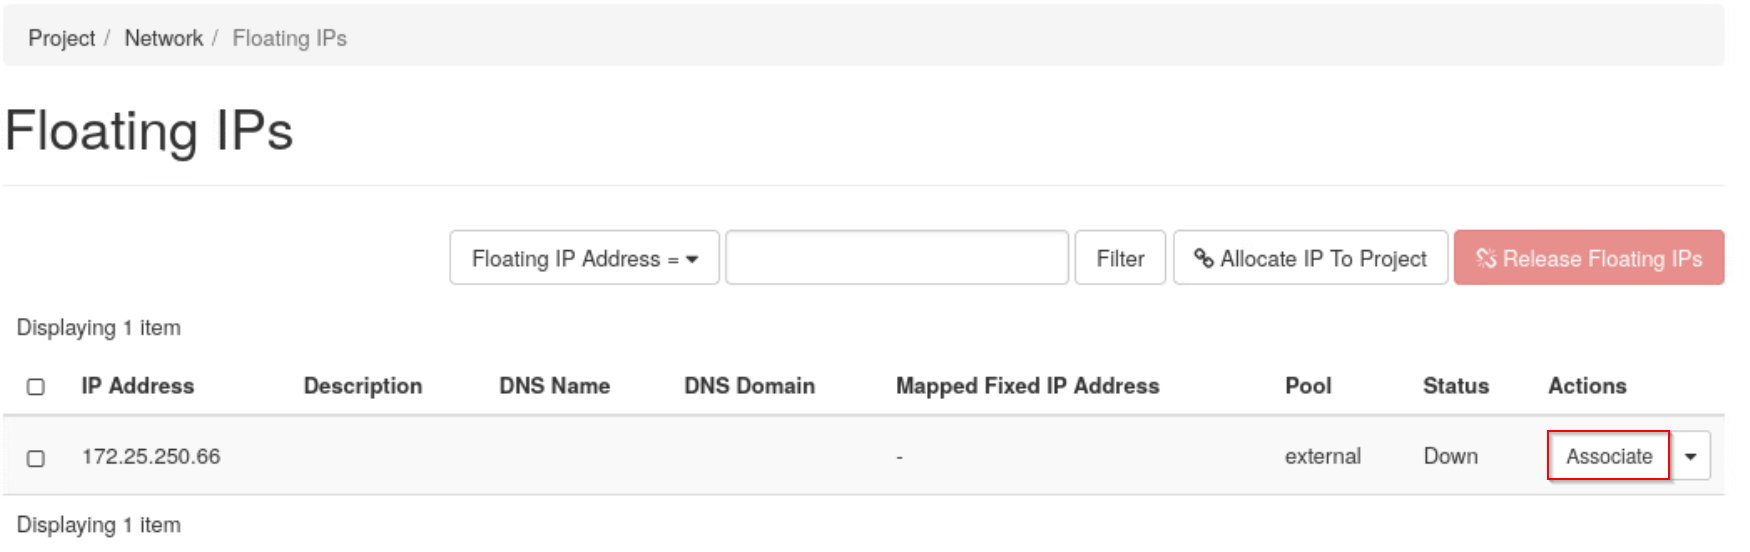
\includegraphics[width=\linewidth]{images/part3/step6.png}
    \end{center}
    
    \begin{notebox}
        The actual value of the floating IP address may differ.
    \end{notebox}

    \item In the \textit{Port to be associated} dropdown, select \textbf{instance1: 192.168.233.XYZ}. Click
    \textbf{Associate}.

    \begin{center}
        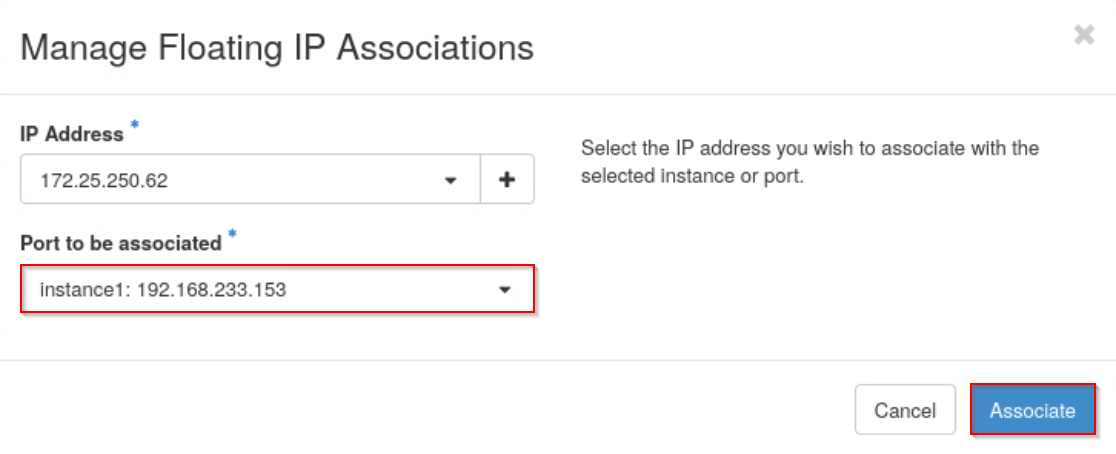
\includegraphics[width=\linewidth]{images/part3/step7.png}
    \end{center}

    \begin{notebox}
        The actual value of the instance's IP address may differ.
    \end{notebox}

    \item The \textbf{instance1} instance is now connected to the \textbf{extern-net2} network through this floating IP
    address. To remove a floating IP address, first navigate to \textbf{Compute $>$ Instances}. Click the arrow next to
    the \textbf{Create Snapshot} in the same as \textbf{instance1}. Select \textbf{Disassociate Floating IP} to detach
    the floating IP from the instance.

    \begin{center}
        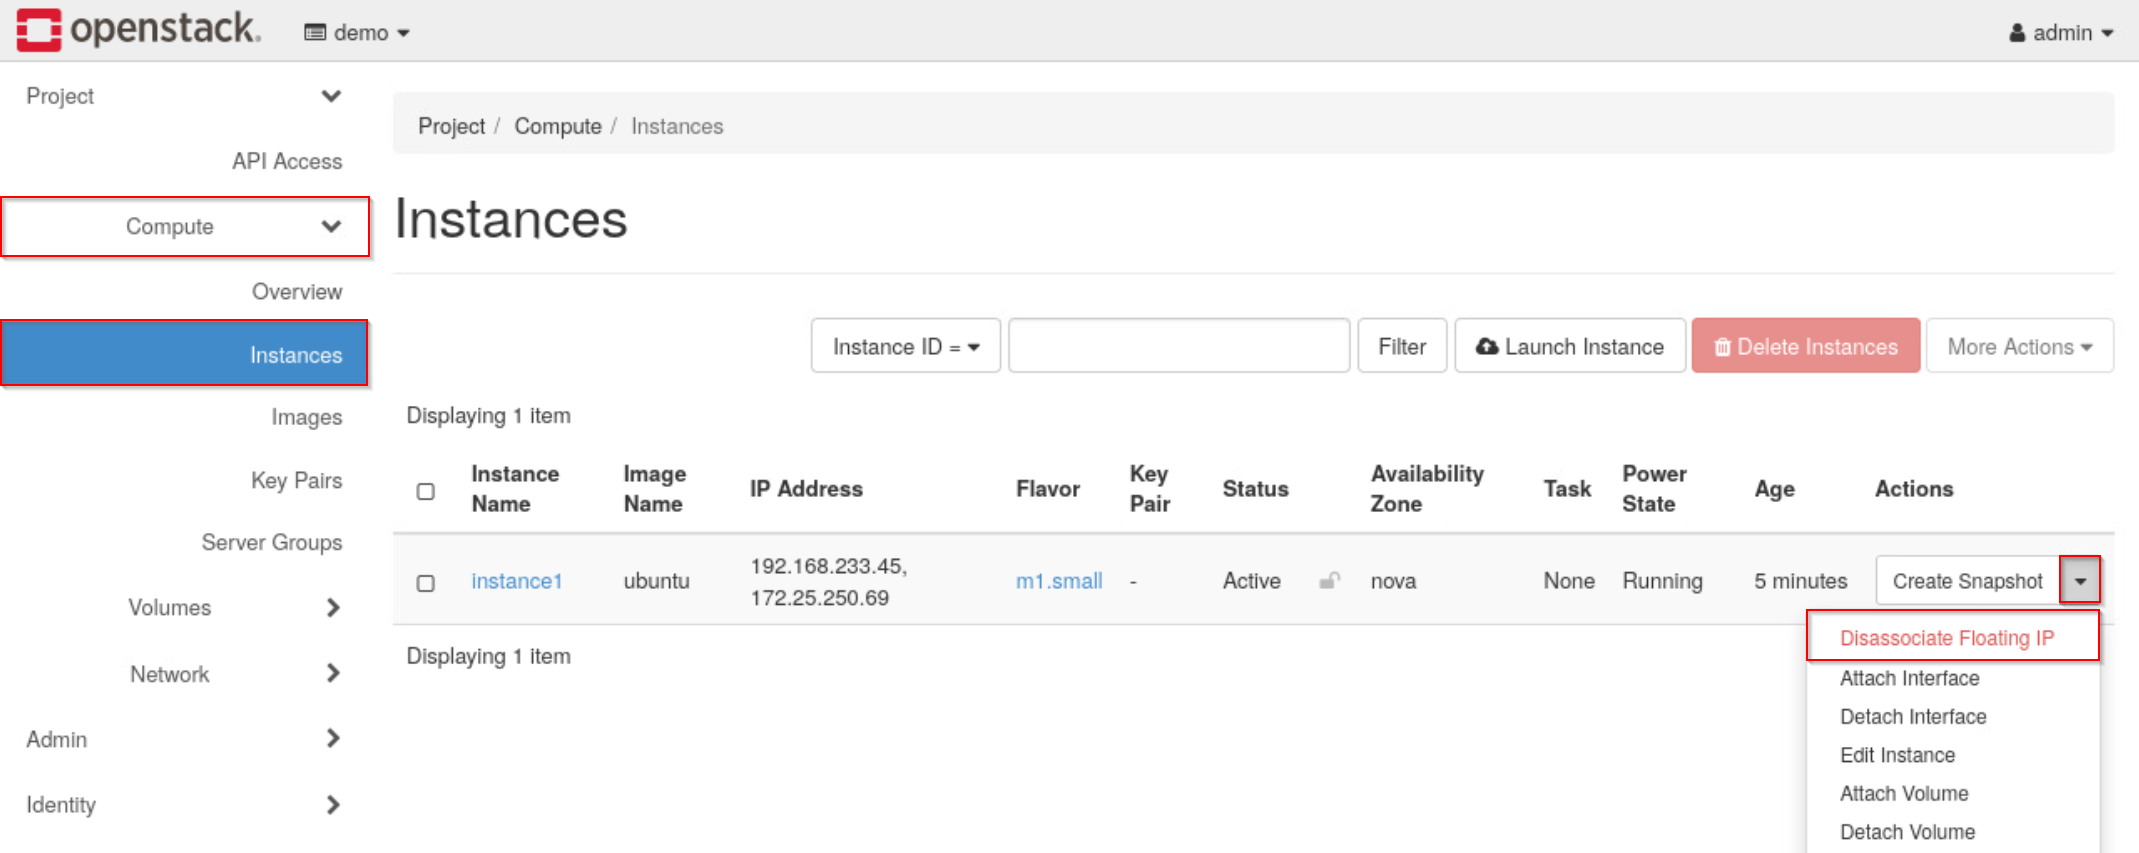
\includegraphics[width=\linewidth]{images/part3/step8.png}
    \end{center}

    \item Check the \textit{Release Floating IP} box and click \textbf{Disassociate}.
    
    \begin{center}
        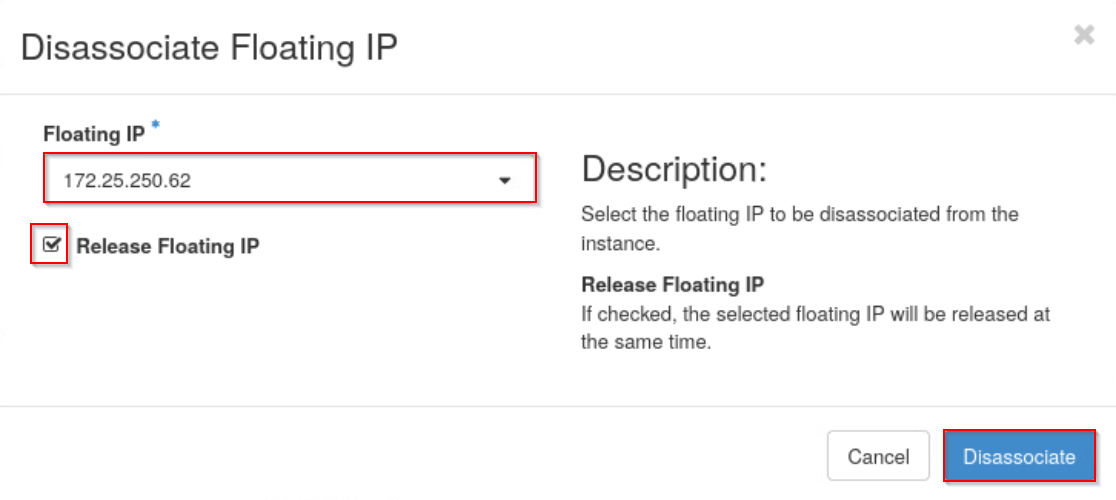
\includegraphics[width=\linewidth]{images/part3/step9.png}
    \end{center}

    \begin{tipbox}
        A floating IP address can also be disassociated from the \textbf{Project $>$ Network $>$ Floating IPs} page.
        When a floating IP address has been associated with an instance, the button in the row of the floating IP
        address that used to read \textbf{Associate} will turn red and read \textbf{Disassociate}. Clicking this button
        will disassociate the floating IP address from its instance.
    \end{tipbox}

    \item Log out of the \textit{Horizon Dashboard} and close the web browser.

    \item From the terminal, allocate a floating IP address in the \textbf{extern-net2} network.
    \begin{lstlisting}
        [ubuntu@workstation (keystone-admin)]:~$ openstack floating ip create \
        > extern-net2
    \end{lstlisting}

    \begin{center}
        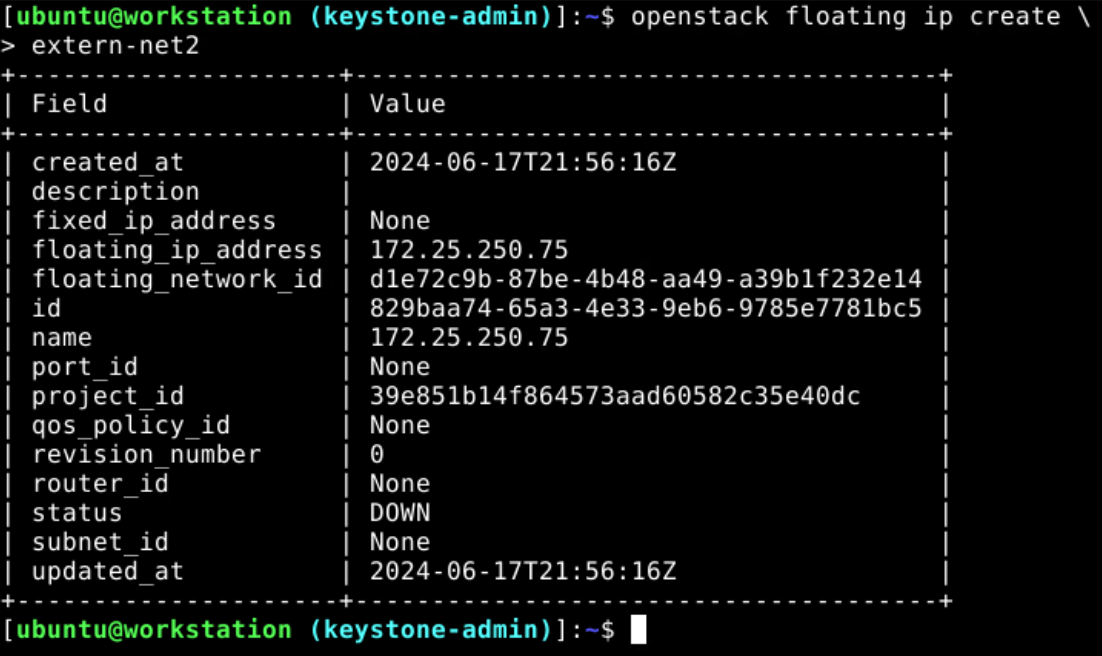
\includegraphics[width=\linewidth]{images/part3/step11.png}
    \end{center}

    \begin{tipbox}
        You can use the \textbf{--floating-ip-address IP\_ADDRESS} argument to allocate a specific IP address.
        However, make sure to list the available addresses before attempting to allocate it. If that particular floating
        IP address already exists, the command will throw an \textit{HttpException: Conflict} error.
    \end{tipbox}
    \begin{tipbox}
        A floating IP address can be disassociated from and instance using the command \textbf{openstack floating ip
        remove INSTANCE FLOATING\_IP\_ADDRESS} and deleted using the command \textbf{openstack floating ip delete
        IP\_ADDRESS}.
    \end{tipbox}

    \item Associate the floating IP with \textbf{instance1}.
    \begin{lstlisting}
        [ubuntu@workstation (keystone-admin)]:~$ openstack server add \
        > floating ip instance1 172.25.250.75
    \end{lstlisting}

    \begin{center}
        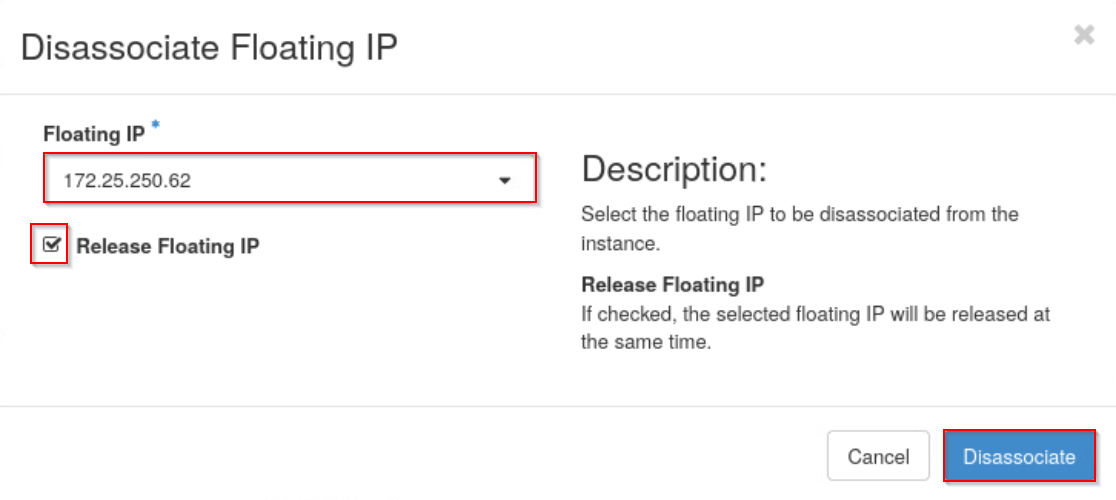
\includegraphics[width=\linewidth]{images/part3/step12.png}
    \end{center}

    \begin{notebox}
        The actual floating IP may differ. Use the floating IP address generated from your output from the previous
        step.
    \end{notebox}

    \item We will recreate this instance at the end of the lab once the rest of the necessary resources have been
    created. We will not need this instance anymore, so delete it. This will also disassociate the floating IP address,
    but it will still be available.
    \begin{lstlisting}
        [ubuntu@workstation (keystone-admin)]:~$ openstack server delete instance1
    \end{lstlisting}

    \item Leave the terminal window open and continue to the next task.

\end{enumerate}

%%%%%%%%%%%
% Section 4
%%%%%%%%%%%
\section{Managing SSH Key Pairs}
\label{sec:managing_ssh_key_pairs}
In this task, you will use the \textit{Horizon Dashboard} and \textit{OpenStack Unified CLI} to manage SSH key pairs
that will be used later in the lab to connect to OpenStack instances from outside of the OpenStack environment.

\begin{enumerate}
    \item Switch to the \textbf{demo} project and navigate to \textbf{Project $>$ Compute $>$ Key Pairs}. Click
    \textbf{Create Key Pair} to create a new key pair.

    \begin{center}
        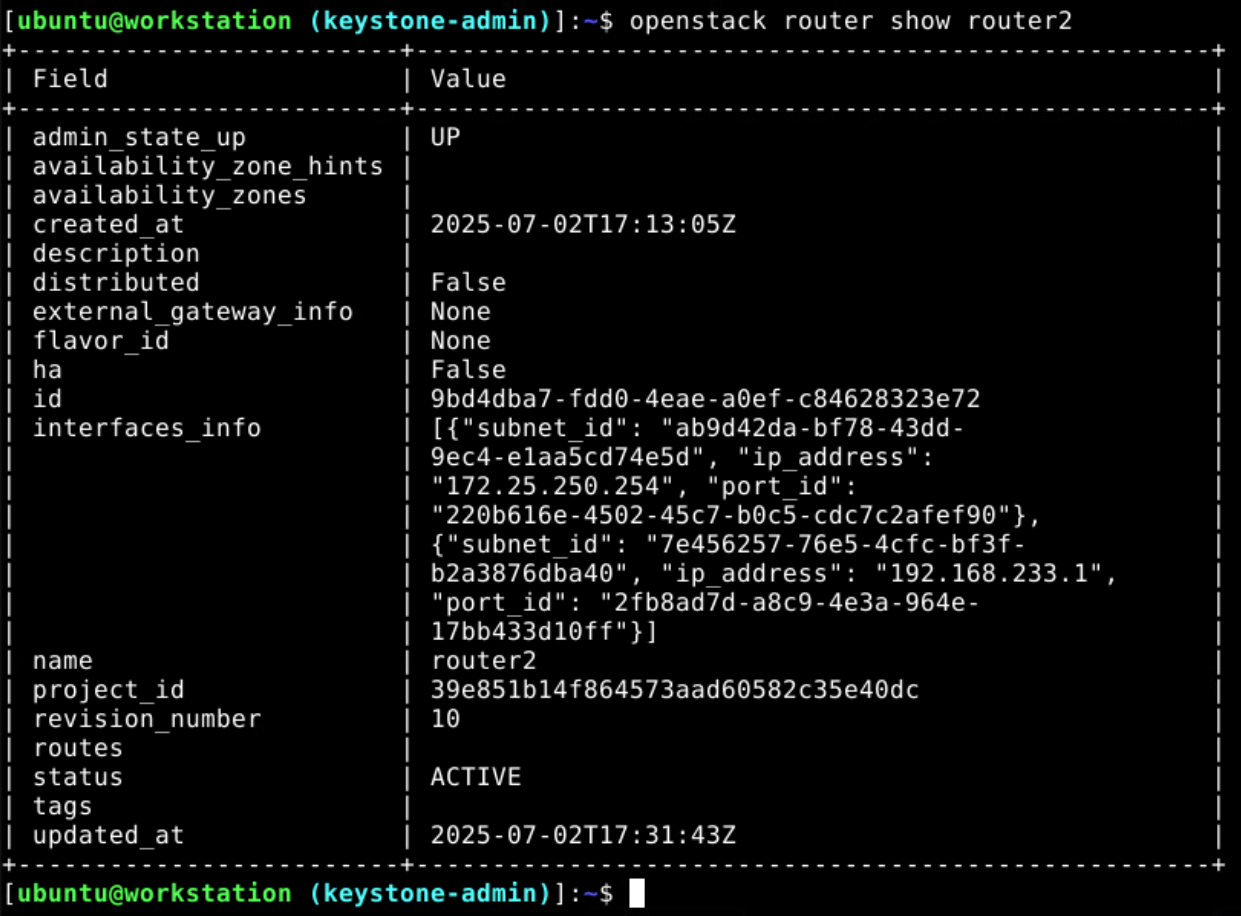
\includegraphics[width=\linewidth]{images/part4/step2.png}
    \end{center}

    \item Enter \textbf{keypair1} in the \textit{Key Pair Name} field, and select \textbf{SSH Key} in the \textit{Key
    Type} dropdown. Click \textbf{Create Key Pair}. This will create the key pair and download it to the
    \textbf{\texttildemid/Downloads} directory.

    \begin{center}
        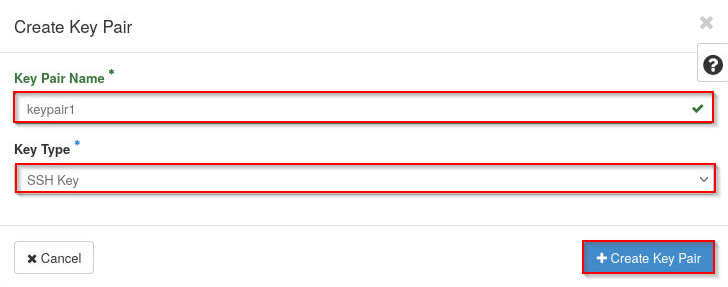
\includegraphics[width=\linewidth]{images/part4/step3.png}
    \end{center}

    \begin{tipbox}
        Key pairs can be deleted from the Horizon Dashboard the same way as other objects. Simply select the checkbox
        next to the key pair you wish to delete, then click \textbf{Delete Key Pairs}.
    \end{tipbox}

    \item Sign out of the Horizon Dashboard and close the web browser.
    
    \item If a terminal window is not already open, open one and source the \textbf{admin} credentials from the
    \textbf{\texttildemid/keystonerc-admin} file.
    \begin{lstlisting}
        ubuntu@workstation:~$ source ~/keystonerc-admin
    \end{lstlisting}

    \begin{center}
        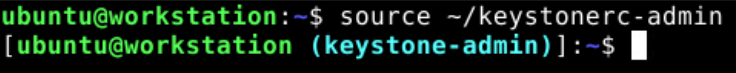
\includegraphics[width=\linewidth]{images/part4/step4.png}
    \end{center}

    \item We only need one key pair to connect to the external instance, so the key pair created from the Horizon
    Dashboard can safely be deleted in order to demonstrate creating a key pair from the command line. Delete the
    \textbf{keypair1} key pair.
    \begin{lstlisting}
        [ubuntu@workstation (keystone-admin)]:~$ openstack keypair delete keypair1
    \end{lstlisting}

    \begin{center}
        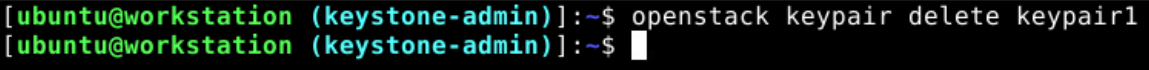
\includegraphics[width=\linewidth]{images/part4/step5.png}
    \end{center}

    \begin{notebox}
        Note that a key pair in the context of OpenStack is actually a misnomer. The key pair object really only refers
        to the public key, while the private key only exists in the file in which it is saved. Therefore, the private
        key file will still exist after deleting the key pair.
    \end{notebox}

    \item Delete the private key located at \textbf{\texttildemid/Downloads/keypair1.pem}.
    \begin{lstlisting}
        [ubuntu@workstation (keystone-admin)]:~$ rm -f ~/Downloads/keypair1.pem
    \end{lstlisting}

    \begin{center}
        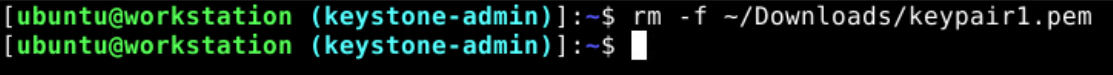
\includegraphics[width=\linewidth]{images/part4/step6.png}
    \end{center}

    \item Create the key pair \textbf{keypair2} and save the private key to the file
    \textbf{\texttildemid/Downloads/keypair2.pem}.
    \begin{lstlisting}
        [ubuntu@workstation (keystone-admin)]:~$ openstack keypair create \
        > keypair2 > ~/Downloads/keypair2.pem
    \end{lstlisting}

    \begin{center}
        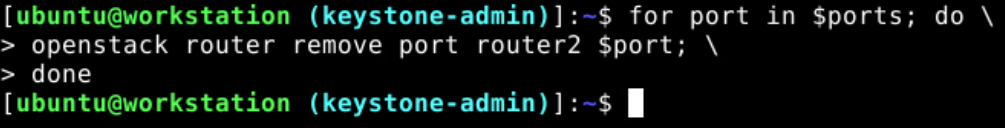
\includegraphics[width=\linewidth]{images/part4/step7.png}
    \end{center}

    \item To better protect the private key, use the \textbf{chmod} command with a mode of \textbf{600} to make it so
    that the \textbf{ubuntu} user has read/write permissions on the private key file, and groups and other users
    have no permissions to the file.
    \begin{lstlisting}
        [ubuntu@workstation (keystone-admin)]:~$ chmod 600 ~/Downloads/keypair2.pem
    \end{lstlisting}

    \begin{center}
        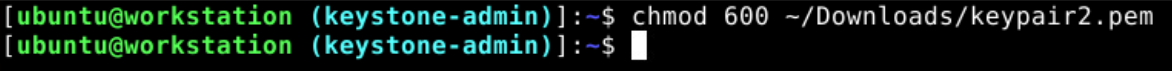
\includegraphics[width=\linewidth]{images/part4/step8.png}
    \end{center}

    \item Leave the terminal window open and continue to the next task.

\end{enumerate}

%%%%%%%%%%%
% Section 5
%%%%%%%%%%%
\section{Implementing Security}
\label{sec:implementing_security}
In this task, you will use the \textit{Horizon Dashboard} and \textit{OpenStack Unified CLI} to manage security groups
for OpenStack instances. This is similar to constructing firewall rules and will be used to allow certain types of
network traffic while disallowing others.

\begin{enumerate}
    \item Open the web browser and navigate to \textbf{192.168.1.20}. Log into the dashboard as \textbf{admin} with the
    password \textbf{secret}.

    \item Switch to the \textbf{demo} project. Navigate to \textbf{Network $>$ Security Groups} and click
    \textbf{Create Security Group}.

    \begin{center}
        \includegraphics[width=\linewidth]{images/part5/step2.png}
    \end{center}

    \item Enter \textbf{secgroup1} into the \textit{Name} field and click \textbf{Create Security Group}.

    \begin{center}
        \includegraphics[width=\linewidth]{images/part5/step3.png}
    \end{center}

    \item After creating the security group, you should land on the page containing the rules for the security group.
    If not, click \textbf{Manage Rules} in the same column as \textbf{secgroup1} on the \textbf{Security Groups} page to
    get there. From here, you can see that by default, the security group allows any egress (outgoing) traffic and does
    not allow any ingress (incoming) traffic. Click \textbf{Add Rule} to add a new rule in the security group.

    \begin{center}
        \includegraphics[width=\linewidth]{images/part5/step4.png}
    \end{center}

    \item Select \textbf{All ICMP} from the \textit{Rule} dropdown and click \textbf{Add}. This will allow ICMP traffic,
    namely the \textbf{ping} command, to reach instances in this security group.

    \begin{center}
        \includegraphics[width=\linewidth]{images/part5/step5.png}
    \end{center}

    \begin{notebox}
        By default, \textit{Direction} is set to \textbf{Ingress} and \textit{CIDR} is set to \textbf{0.0.0.0/0}.
        \textbf{Ingress} specifies incoming traffic, and \textbf{0.0.0.0/0} specifies that the traffic is accepted from
        any IP address.
    \end{notebox}

    \item Log out of the \textit{Horizon Dashboard} and close the web browser.
    
    \item If a terminal window is not already open, open one and source the \textbf{admin} credentials from the
    \textbf{\texttildemid/keystonerc-admin} file.
    \begin{lstlisting}
        ubuntu@workstation:~$ source ~/keystonerc-admin
    \end{lstlisting}

    \begin{center}
        \includegraphics[width=\linewidth]{images/part5/step7.png}
    \end{center}

    \item Next, we will recreate this security group through the command line and add some additional rules necessary
    for connecting to an external instance. First, to demonstrate how to remove a rule from a security group, list the
    rules in the \textbf{secgroup1} security group and copy the ID of the ICMP rule.
    \begin{lstlisting}
        [ubuntu@workstation (keystone-admin)]:~$ openstack security group rule list \
        > secgroup1
    \end{lstlisting}

    \begin{center}
        \includegraphics[width=\linewidth]{images/part5/step8.png}
    \end{center}

    \begin{tipbox}
        To copy a value from the terminal, select the desired string with the mouse, then either right-click and click
        \textbf{Copy} or press press \textbf{Ctrl+Shift+C}. 
    \end{tipbox}

    \item Use the \textit{ID} for the ICMP rule to delete that rule.
    \begin{lstlisting}
        [ubuntu@workstation (keystone-admin)]:~$ openstack security group rule delete \
        > ceeea025d-60f2-440a-a471-ea876e6857bd
    \end{lstlisting}

    \begin{center}
        \includegraphics[width=\linewidth]{images/part5/step9.png}
    \end{center}

    \begin{notebox}
        The actual ID value may differ.
    \end{notebox}
    \begin{tipbox}
        To paste a value to the command line, either right-click and click \textbf{Paste} or press
        \textbf{Ctrl+Shift+V}.
    \end{tipbox}

    \item List the rules in the \textbf{secgroup1} security group again to ensure the rule was deleted successfully.
    \begin{lstlisting}
        [ubuntu@workstation (keystone-admin)]:~$ openstack security group rule list \
        > secgroup1
    \end{lstlisting}

    \item Delete the \textbf{secgroup1} security group.
    \begin{lstlisting}
        [ubuntu@workstation (keystone-admin)]:~$ openstack security group delete \
        > secgroup1
    \end{lstlisting}

    \begin{center}
        \includegraphics[width=\linewidth]{images/part5/step11.png}
    \end{center}

    \item Create the \textbf{secgroup2} security group.
    \begin{lstlisting}
        [ubuntu@workstation (keystone-admin)]:~$ openstack security group create \
        > --max-width 80 secgroup2
    \end{lstlisting}

    \begin{center}
        \includegraphics[width=\linewidth]{images/part5/step12.png}
    \end{center}

    \item List the rules in the \textbf{secgroup2} security group. These are the default rules that exist upon
    creation.
    \begin{lstlisting}
        [ubuntu@workstation (keystone-admin)]:~$ openstack security group rule list \
        > secgroup2
    \end{lstlisting}

    \begin{center}
        \includegraphics[width=\linewidth]{images/part5/step13.png}
    \end{center}

    \begin{tipbox}
        You can use the command \textbf{openstack security group rule show RULE\_ID} to show the details of each rule
        and confirm that they are the same default rules you get when creating a security group throug the Horizon
        Dashboard. The rules allow all outgoing traffic over IPv4 and IPv6.
    \end{tipbox}

    \item Add a security rule in the \textbf{secgroup2} security group to allow all incoming ICMP traffic. 
    \begin{lstlisting}
        [ubuntu@workstation (keystone-admin)]:~$ openstack security group rule create \
        > --protocol icmp \
        > secgroup2
    \end{lstlisting}

    \begin{center}
        \includegraphics[width=\linewidth]{images/part5/step14.png}
    \end{center}

    \begin{notebox}
        If no arguments are given, the direction defaults to \textbf{ingress} and the remote IP defaults to
        \textbf{0.0.0.0/0}. In other words, it allows all incoming traffic over the given protocol.
    \end{notebox}

    \item List the rules in the \textbf{secgroup2} security group again to ensure the ICMP rule was created
    successfully.
    \begin{lstlisting}
        [ubuntu@workstation (keystone-admin)]:~$ openstack security group rule list \
        > secgroup2
    \end{lstlisting}

    \item Add another security rule to allow remote connection using SSH on the default port 22.
    \begin{lstlisting}
        [ubuntu@workstation (keystone-admin)]:~$ openstack security group rule create \
        > --protocol tcp \
        > --dst-port 22 \
        > secgroup2
    \end{lstlisting}

    \begin{center}
        \includegraphics[width=\linewidth]{images/part5/step16.png}
    \end{center}

    \item List the rules in the \textbf{secgroup2} security group again to ensure the SSH rule was created
    successfully.
    \begin{lstlisting}
        [ubuntu@workstation (keystone-admin)]:~$ openstack security group rule list \
        > secgroup2
    \end{lstlisting}

    \item Leave the terminal window open and continue to the next task.

\end{enumerate}

%%%%%%%%%%%
% Section 6
%%%%%%%%%%%
\section{Launching and Verifying an External Instance}
\label{sec:launching_an_external_isntance}
Up to this point, we have created an external network, a router, a floating IP address, an SSH key pair, and a security
group. These are all the resources necessary to create and interact with an external instance from outside the OpenStack
cloud. In this task, you will launch an external instance and verify its connectivity and functionality using the
\textbf{ssh} and \textbf{ping} commands.

\begin{enumerate}
    \item If a terminal window is not already open, open one and source the admin credentials from the 
    \textbf{\texttildemid/keystonerc-admin} file.
    \textbf{\texttildemid/keystonerc-admin} file.
    \begin{lstlisting}
        ubuntu@workstation:~$ source ~/keystonerc-admin
    \end{lstlisting}

    \begin{center}
        \includegraphics[width=\linewidth]{images/part6/step1.png}
    \end{center}

    \item List all instances in the project. The list should be empty.
    \begin{lstlisting}
        [ubuntu@workstation (keystone-admin)]:~$ openstack server list
    \end{lstlisting}

    \begin{center}
        \includegraphics[width=\linewidth]{images/part6/step2.png}
    \end{center}

    \item Launch an instance named \textbf{instance-external} using the \textbf{ubuntu} image, the \textbf{m1.small}
    flavor, the \textbf{keypair2} key pair, the \textbf{shared} network, and the \textbf{secgroup2} security
    group.
    \begin{lstlisting}
        [ubuntu@workstation (keystone-admin)]:~$ openstack server create \
        > --image ubuntu \
        > --flavor m1.small \
        > --key-name keypair2 \
        > --nic net-id=shared \
        > --security-group secgroup2 \
        > instance-external
    \end{lstlisting}

    \begin{center}
        \includegraphics[width=\linewidth]{images/part6/step3.png}
    \end{center}

    \item List the floating IPs.
    \begin{lstlisting}
        [ubuntu@workstation (keystone-admin)]:~$ openstack floating ip list \
        > --max-width 90
    \end{lstlisting}

    \begin{center}
        \includegraphics[width=\linewidth]{images/part6/step4.png}
    \end{center}

    \item Associate the floating IP address with the \textbf{instance-external} instance.
    \begin{lstlisting}
        ubuntu@workstation;~$ openstack server add floating ip \
        > instance-external 172.25.250.75
    \end{lstlisting}

    \begin{center}
        \includegraphics[width=\linewidth]{images/part6/step5.png}
    \end{center}

    \begin{notebox}
        Be sure to use the floating IP address that matches your output as they may differ slightly from this example.
    \end{notebox}

    \item Verify that the instance was assigned the floating IP address.
    \begin{lstlisting}
        [ubuntu@workstation (keystone-admin)]:~$ openstack server list \
        > -c Name \
        > -c Networks
    \end{lstlisting}

    \begin{center}
        \includegraphics[width=\linewidth]{images/part6/step6.png}
    \end{center}

    \begin{tipbox}
        For commands that output tables, you can pull out only the columns you want by using the \textbf{-c} option
        followed by the column name. This option can be chained as in the command above to list multiple columns.
    \end{tipbox}

    \item Use the \textbf{scp} command to send the \textbf{keypair2} key pair to the \textbf{devstack} machine using
    the SSH protocol. Use the password \textbf{ubuntu} for authentication.
    \begin{lstlisting}
        [ubuntu@workstation (keystone-admin)]:~$ scp ~/Downloads/keypair2.pem \
        > ubuntu@192.168.1.20:~/keypair2.pem
    \end{lstlisting}

    \begin{center}
        \includegraphics[width=\linewidth]{images/part6/step7.png}
    \end{center}

    \item SSH into the \textbf{devstack} machine. Use the password \textbf{ubuntu} when prompted.
    \begin{lstlisting}
        [ubuntu@workstation (keystone-admin)]:~$ ssh 192.168.1.20
    \end{lstlisting}

    \begin{center}
        \includegraphics[width=\linewidth]{images/part6/step8.png}
    \end{center}

    \item Ping the \textbf{external-instance} instance using the floating IP that was assigned to it in the previous
    task.
    \begin{lstlisting}
        ubuntu@devstack:~$ ping -c3 172.25.250.75
    \end{lstlisting}

    \begin{center}
        \includegraphics[width=\linewidth]{images/part6/step9.png}
    \end{center}

    \begin{notebox}
        You should receive three successful ping replies.
    \end{notebox}

    \item SSH into the \textbf{instance-external} instance, using the \textbf{keypair2.pem} file to authenticate. Enter
    \textbf{yes} when asked if you want to continue.
    \begin{lstlisting}
        ubuntu@devstack:~$ ssh -i ~/keypair2.pem \
        > 172.25.250.75
    \end{lstlisting}
 
    \begin{center}
        \includegraphics[width=\linewidth]{images/part6/step10.png}
    \end{center}

    \begin{notebox}
        It may take a few minutes for the instance to be fully booted and ready to accept SSH connections.
    \end{notebox}
    \begin{notebox}
        It is important to connect to the instance through SSH from the \textbf{devstack} machine since it is outside of
        the OpenStack cloud. A successful connection verifies the external connectivity of the instance.
    \end{notebox}

    \item Ping the DHCP server on the \textbf{shared} network to verify connectivity.
    \begin{lstlisting}
        ubuntu@instance-external:~$ ping -c3 192.168.233.2
    \end{lstlisting}

    \begin{center}
        \includegraphics[width=\linewidth]{images/part6/step11.png}
    \end{center}

    \begin{notebox}
        You should receive three successful ping replies.
    \end{notebox}

    \item The lab is now complete.

\end{enumerate}
\end{document}
